\documentclass{ieeeaccess}
\usepackage[nobreak]{cite}
\usepackage{amsmath, amssymb, amsfonts}
\usepackage{algorithmic}
\usepackage{graphicx}
\usepackage{textcomp}
\usepackage{array}
\usepackage{booktabs}
\usepackage{longtable} % 長い表を扱うためのパッケージ
\usepackage{multirow}
\usepackage{colortbl}
\usepackage{tabularx}
\usepackage{graphicx}
\usepackage{pdflscape}
\usepackage[margin=1in]{geometry}
\usepackage{graphicx}
\usepackage{colortbl}
\usepackage{hhline}
\usepackage[export]{adjustbox}
\usepackage{url}
\usepackage{rotating}
\definecolor{pink}{rgb}{1,0.75,0.8} % ピンク色を定義

\begin{document}
    \history{Date of publication xxxx 00, 0000, date of current version xxxx 00, 0000.}
    \doi{10.1109/ACCESS.2017.DOI}

    \title{Does multi-day motor imagery EEG data validate reproducibility and enable generalized discrimination algorithms?}
    \author{\uppercase{Yuminosuke Sato}\authorrefmark{1}, \uppercase{Yuichi
    Yaguchi}\authorrefmark{2}}

    \address[1]{University of Aizu, Fukushima Japan (e-mail: m5261158@u-aizu.ac.jp)}
    \address[2]{University of Aizu, Fukushima Japan (e-mail: yaguchi@u-aizu.ac.jp)}

    \markboth {Author \headeretal: Preparation of Papers for IEEE TRANSACTIONS and JOURNALS}
    {Author \headeretal: Preparation of Papers for IEEE TRANSACTIONS and JOURNALS}


    \begin{abstract}
        We investigate reproducibility and generalizability of motor imagery (MI)-based electroencephalography (EEG) signals. A multi-day consumer-grade MI-EEG dataset with 25 subjects was used to examine long-term EEG consistency. The outcomes of four EEG verification techniques were compared, namely, tri-dataset verification (TDV), dual-dataset verification (DDV), temporal verification (TV), and subject dependent tri-dataset verification (SDTDV). Results showed that incorporating some test-day data for model adaptation (DDV) yielded higher accuracy than solely using pre-trained models (TDV). Test-day training alone (TV) also exhibited competitive performance in some metrics. The outcomes verify the reproducibility of MI-EEG across days, demonstrating that generalized discrimination algorithms can effectively categorize individual EEG patterns. This study pioneers an approach to evaluating the real-world effectiveness of MI-EEG systems, enabling translation of this technology into assistive applications. The source code can be found at \url{https://github.com/Buddies-as-you-know/EEG_classification}.
    \end{abstract}

    \begin{keywords}
        Brain-Computer Interfaces (BCI), Electroencephalography (EEG), End-to-End
        Learning, Motor Imagery (MI), Performance Evaluation, Signal Classification
    \end{keywords}

    \titlepgskip=-15pt

    \maketitle

    
    \section{INTRODUCTION}
\label{sec:introduction}
Brain-computer interface (BCI) technology represents a groundbreaking approach, deciphering the brain's motor imagery (MI) to issue commands without necessitating physical movement\cite{benzy2020motor}. This technology is particularly promising as it activates the same neural pathways when imagining a movement like those used during actual movement execution, offering an alternative modality of action for individuals with mobility loss\cite{guillot2009brain}. For example, it opens doors to alternative locomotive methods, such as prosthetic limbs and robotic arms\cite{gupta2020prototype,korik2019decoding,cho2021neurograsp}. Anticipated to reduce fatigue, BCI technology heralds a new paradigm in assistive living\cite{lotze2006motor,mulder2007motor}. Research in MI-EEG is pivotal in advancing medical and assistive technologies, with its progress expected to further catalyze technological innovations.


MI represents a critical cognitive process in both neuroscience and sports psychology\cite{bovend2012practical,cryder2023guided}. It involves the mental simulation of a physical action without its actual execution. This process activates the brain regions associated with motor control and planning\cite{henschke2023engaging,munzert2009cognitive} Such activation mirrors the neural patterns observed during the physical performance of the action.

\vspace{3mm}

The significance of MI lies in its application across various fields. In sports, athletes use it to enhance their performance by mentally rehearsing specific skills\cite{cederstrom2021effect,app12199753}. In rehabilitation, it aids individuals with motor impairments in regaining movement capabilities. Furthermore, MI serves as a tool for understanding the neural mechanisms underlying motor control and learning\cite{tong2017motor, choy2023virtual}.

\vspace{3mm}
The utilization of MI-based EEG classification in a variety of applications,
such as unmanned aerial vehicle (drone) operation, motorized wheelchairs,
navigation systems in humanoid robots, and the functioning of artificial limbs,
necessitates real-time identification that is crucial for the operational efficacy
of these technologies\cite{zhang2018converting,chaudhary2020flexible,huang2019eeg,dumitrescu2021using}. Particularly in the case of drones and electric vehicles,
combination of heightened situational awareness and adept operation is
imperative\cite{liu2020parallel,freitas2019real}. The fidelity of MI-based EEG recognition, requiring both high precision and swift responsiveness, plays a pivotal role due to its direct implications on user safety and the functional proficiency of the technology\cite{liu2017identification}. Thus, enhancement of the reproducibility and reliability of MI-EEG technology is of paramount importance in its development for practical applications.

\vspace{3mm}

This research endeavors to authenticate the reproducibility of motor imagery
(MI)-based electroencephalography (EEG) datasets and the universality of the
discrimination algorithm utilized\cite{zhang2018converting,chaudhary2020flexible,huang2019eeg,dumitrescu2021using}. Traditional EEG investigations have
predominantly concentrated on elevating data precision and optimizing
electrode placement, exemplified by endeavors to transcend the state-of-the-art
(SOTA) in discrimination accuracy in BCI competitions etc\cite{du2023recognition,deng2021advanced,xu2019deep,suemitsu2023effects, sharma2023recent}. Nonetheless, within practical environments, the emphasis shifts to the steadfastness of data
reproducibility and the all-encompassing applicability of the model\cite{nakamura2017ear}. For instance,
MI-based EEG outputs must remain consistent for identical
commands executed by the same subject, irrespective of variations in temporal
and environmental contexts. Similarly, the precision in identifying MI-based
EEG patterns ought to maintain uniformity across differing scenarios. This
study not only scrutinizes the reproducibility and universal applicability
of MI-based EEGs but also aims to significantly enhance the interpretative
breadth and practical deployment of EEG data.


\vspace{3mm}

This investigation delves into the consistency of EEG data reproducibility across various days and among different subjects. The process
of data gathering over extended periods could potentially compromise the uniformity
of the data, as result of factors such as electrode displacement and
intrinsic physiological variances. It is of paramount importance to evaluate
the reproducibility to ascertain EEG's dependability in pragmatic scenarios,
especially considering the impracticality of employing consumer-grade BCIs or the elimination of electrooculograms (EOG) in real-world
applications. The primary objective of this assessment is to ascertain the steadfastness
of MI-based EEG data and the universal applicability of the recognition
models employed. Adopting this methodology could substantially enhance both
the utility and dependability of EEG data for broader applications.


\vspace{3mm}
This investigation scrutinizes the efficacy of extant discrimination models
when applied to novel environments, disparate subjects, and over extended
durations. Predominant models often exhibit heightened accuracy solely in specific,
controlled conditions, exemplified by the results seen in the BCI competition
(as seen in Table \ref{tab: Comparison of existing data sets and the data sets used in this study}). The crux of this study is to validate the universality
of these models by evaluating their adaptability to new, diverse datasets.
Such validation is crucial for confirming the practical effectiveness of EEG-based
systems in real-world scenarios. Consequently, this research offers
innovative directions in both the analytical and practical application of
EEG data. In contrast to traditional EEG research, which is primarily focused on
idealized experimental conditions, this study pioneers in exploring the reproducibility
of EEG data and the universal applicability of models within more realistic settings.
This novel approach is anticipated to significantly bolster the utility and
reliability of EEG technology in actual applications. Ultimately, this study
carves a new path in EEG research, heralding an era of more grounded and practical
applications. Our main contributions are as follows:
\begin{itemize}
    \vspace{1mm}
    \item We investigated EEG consistency over time using a multi-day consumer-grade MI-EEG dataset including 25 subjects.
    \vspace{3mm}
    \item Through a comparison of EEG validation techniques (TDV, DDV, TV, SDTDV), we showed that using a portion of the test day data for model adaptation can yield higher accuracy than using only a pre-trained model. .
    \vspace{3mm}
    \item We confirmed the daily reproducibility of MI-EEG and verified the effectiveness of a generalized identification algorithm that can effectively classify individual EEG patterns.
    \vspace{3mm}
    \item We have pioneered a new approach to evaluating the effectiveness of MI-EEG systems in the real world, making it possible to translate this technology into assistive applications.
    \vspace{3mm}
    \item We made the source code public to improve the reproducibility and transparency of our research.
\end{itemize}
    \section{RELATED WORK}
\label{sec:relatedwork}
    \subsection{MI-EEG APPLICATIONS and ROBOTICS}
    \label{subsec:MI-EEG APPLICATIONS and ROBOTICS}
        \subsubsection*{Importance of Real-time Responsiveness and Reproducibility in MI-EEG}
        Efficacy of MI-based EEG  in practical applications hinges on its real-time responsiveness and reproducibility. Real-time operation is critical for immediate and accurate execution of user intentions, while reproducibility ensures consistent performance across different sessions and users. These attributes are paramount in applications where user safety and operational efficiency are at stake \cite{singh2021comprehensive}.

        \subsubsection*{Application in Unmanned Aerial Vehicles (Drones)}
        \label{subsubsec:Application in Unmanned Aerial Vehicles (Drones)}
        Integration of MI-EEG into drone technology will enable people who cannot move their limbs to operate them. This advancement enables real-time operation using brain signals, which is essential in dynamic and unpredictable environments. The repeatability of these brain signal interpretations is crucial for consistent and safe drone navigation. In this way, MI-EEG contributes to both innovation and operational proficiency in drone technology\cite{dumitrescu2021using}.

        \subsubsection*{Use in Motorized Wheelchairs}
        \label{subsubsec:Use in Motorized Wheelchairs}
        In motorized wheelchairs, MI-EEG facilitates realtime movement control, transforming the lives of individuals with mobility impairments \cite{palumbo2021motor,wang2024mi}. The reproducibility of signal interpretation is essential for ensuring consistent and safe wheelchair operation. This technology's realtime responsiveness and reliability significantly enhance user autonomy and mobility.

        \subsubsection*{Application in Humanoid Robot Navigation}
        \label{subsubsec:Application in Humanoid Robot Navigation}
        Humanoid robots equipped with MI-EEG systems offer realtime control through thought, which is essential in navigating complex and hazardous environments\cite{aljalal2019robot}. The reproducibility of these systems is vital for ensuring precise and safe robot maneuvering. Therefore, MI-EEG's reliability and realtime operation extend the functionality and utility of humanoid robots in critical applications.

        \subsubsection*{Functioning of Artificial Limbs}
        In artificial limbs, MI-EEG technology enables real-time movement mimicry and signal interpretation \cite{al2018eeg}. The consistency of these interpretations is crucial for user safety and seamless limb operation. Thus, the reproducibility and real-time responsiveness of MI-EEG are key factors in improving the quality of life for amputees.

    The integration of MI-EEG technology in various applications emphasizes its potential to enhance operational efficiency and quality of life. The importance of real-time responsiveness and reproducibility in these applications underlines the technology's capability to ensure user safety and consistent performance.
    \subsection{MI EEG DATASET}
    Table \ref{tab: Comparison of existing data sets and the data sets used in this study}. show that ma2022\cite{ma2022large} has substantive advantages over other major MI-EEG datasets, in terms of scale and duration. With 25 subjects, ma2022\cite{ma2022large} has over double the next largest cohort of 14 in BNCI2015\_001\cite{faller2012autocalibration} and 54 in Lee2019\_MI\cite{lee2019eeg}. Moreover, it includes multi-day data spanning 5 days, while most datasets recorded single sessions. In terms of duration, are BNCI2014\_004\cite{leeb2007brain}, BNCI2015\_004\cite{scherer2015individually}, and Zhou2016\cite{zhou2016fully} with 2--3 days. However, these data sets have 9, 9, and 4 participants, respectively, and the 25 participants in ma2022 are larger. Additionally, ma2022 uniquely uses consumer-grade BCI devices, making it more accessible and usable for real-world applications. By contrast, nearly all other datasets relied on complex medical-grade equipment. Thus, the table highlights ma2022 as a leader, in terms of participant size, longitudinal span, and practicality through its innovative consumer-grade BCI focus over multiple days.

    The ma2022 dataset has three distinguishing characteristics: adoption of consumer-grade BCI devices, multi-day EEG recordings, and a substantial subject cohort. With 25 participants across 5 days, it has the most extensive longitudinal multi-day data crucial for accounting for EEG signal variability. It uses affordable consumer BCI systems rather than intricate, high-end medical equipment.

    By contrast, the existing datasets employ medical devices and single-day recordings with smaller samples. Its scale and duration uniquely distinguish ma2022 to enable richer insights into EEG patterns over time. Additionally, the pragmatic consumer-grade BCI facilitates applications like drone control requiring minimal intrusive gear.

    The exceptionally large participant pool analyzed longitudinally qualifies ma2022 as an inclusive, pragmatic basis for MI-EEG investigation with advantages over current datasets constrained to medical devices and isolated recordings. It promises deeper revelations into EEG behavior through sizable, multi-day data grounded in easily accessible consumer BCIs usable for real-world problems.
    \subsection{MULTIPLE DAY EEG VALIDATION}
    In the evolving field of BCI research, our study introduces innovative methods to enhance model adaptability and generalization using multi-day MI-based EEG data. Unlike the method by Amjad Abu-Rmileh\cite{kaya2023identifying}, which employs Linear Discriminant Analysis(LDA) Classifier for 18 subjects over four days, our approach involves a more extensive participant base of 25 subjects across the same number of days. This broader subject range is crucial for enhancing the reliability and generalizability of our findings. While Abu-Rmileh's study focuses on EEG power spectrum feature extraction, our method does not utilize feature extraction, distinguishing it in methodology. The objective of Abu-Rmileh's research is to improve BCI training effectiveness, whereas our study concentrates on reproducibility verification.

    In contrast to Esra Kaya's study, which involves an in-depth analysis of a single subject over 20 days using an Ensemble Subspace Discriminant Classifier~\cite{abu2019co}, our research utilizes advanced neural network models. Kaya's study emphasizes optimal channel finding through extensive feature extraction including time, frequency and spatiotemporal and nonlinear features. However, our study diverges by not employing traditional feature extraction techniques, focusing instead on leveraging the inherent capabilities of convolutional networks, transformers, and graph networks. This divergence in approach is a significant differentiator, contributing to our research's uniqueness in the field.

    Comparing our methods with the ma2022 study, which uses a variety of algorithms like Common Spatial Patterns (CSP), Filter Bank Common Spatial Pattern (FBCSP), and adaptive transfer learning for 25 subjects over five days~\cite{ma2022large}, our study similarly involves 25 subjects within the same time frame. However, ma2022's focus on improving cross-session classification in BCI contrasts with our objective of reproducibility verification. Both studies share a commitment to open-access datasets, which is a positive trend toward transparency and collaborative research in the field. However, our research stands out by not relying on feature extraction algorithms, a commonality in ma2022's methodology, and instead opts for a more holistic approach using advanced neural networks.

    In summary, our research introduces a novel approach to BCI studies, emphasizing a larger participant base and advanced neural network models without traditional feature extraction. This methodology sets our research apart from existing studies, contributing uniquely to the field's understanding of model adaptability and generalization in the context of multi-day MI-EEG data.
    \begin{figure*}[tb]
        \centering
        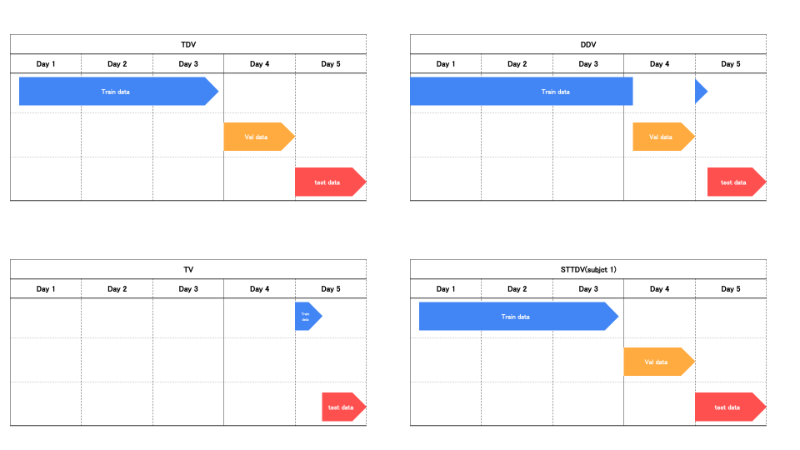
\includegraphics[width=1\linewidth, height=0.5\textheight]{validation.png}
        \caption{Comparison of TDV, DDV, TV, and SDTDV: Model Evaluation Strategy using Day 5 as the Test Day. \newline
        TDV trains the model on four days of pre-training data and evaluates the model's classification performance on day 5 data. DDV adjusts the pre-training model using 
        the first 20\% of the day 5 data and evaluates model performance using the test day data. TV validates the effectiveness of the model without pre-training by training
        using only the first 20\% of the data and assessing performance with the remaining 80\%.
        SDTDV uses four days of pre-training data for each subject and the test data on day 5 
        to evaluate effectiveness.}
        \label{fig: COMPARISON OF THE PROPOSED VERIFICATION TECHNIQUES if day 5 is a test}
    \end{figure*}
    \begin{figure*}[tb]
        \centering
        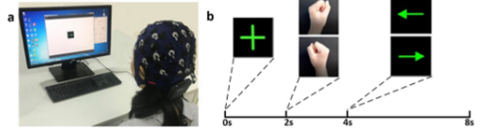
\includegraphics[width=1\linewidth]{a15.png}
        \caption{Data acquisition scenario. Informed consent was obtained from the individual in the figure for the publication of the images \cite{ma2022large}.}
        \label{fig:Data acquisition scenario. Informed consent was obtained from the individual in the figure for the publication of the images}}
    \end{figure*}

    

\section{METHOD}
\subsection{DATASET DESCRIPTION AND SUBJECT}
This study used the extensive and publicly available MI-BCI EEG database, which
consists of five sessions of EEG recordings from 25 participants(13 males
and 12 females; age range, 20–24 years) over 2–3 days. Each session
comprised 100 MI grasping trials with the left and right hands, lasting approximately
7.5 s. Human data collection was approved by the Shanghai Second
Rehabilitation Hospital Ethics Committee (approval No.: ECSHSRH 2018-0101)
under the Declaration of Helsinki. Participants were instructed to imagine
a grasping motion with their left and right hands, guided by visual and
auditory cues. Dynamic MI tasks were recorded using 32 EEG electrodes with an
impedance level of less than $20 k\Omega$ and a sampling frequency of 250 Hz
\cite{ma2022large}. The data preprocessing steps include removing bad segments based on
amplitude thresholding and visual inspection, band-pass filtering with a
0.5--40 Hz finite impulse response filter, and baseline removal.
\subsection{BASE MODEL}
This study employed an end-to-end learning method for MI-based EEG signal
classification. This method was chosen because it increases the systems robustness
and can potentially eliminate outliers and other errors affected by the analyst.
As classifiers, we employed EEG-Inception \cite{zhang2021eeg}, EEGNet \cite{lawhern2018eegnet}, and Schirrmeister
et al.s \cite{schirrmeister2017deep} deep convolutional network (DevConv) models, which are capable
of real-time discrimination with a limited number of electrodes. These models
can be also efficiently trained with a smaller number of channels. As a
baseline for the discriminations obtained with these learning methods, we also
showed the results from assigning random labels to the binary discriminations
for the input.

\subsubsection{EEG-Inception}
The EEG-Inception model is a convolutional neural network architecture that consists
of multiple inception modules, which are designed to capture multi-scale and
multi-level features from EEG signals. The inception module is composed of
parallel convolutional layers with different filter sizes and pooling
operations, followed by concatenation of their outputs. The EEG-Inception
model also includes batch normalization, dropout, and global average pooling
layers to improve the model's generalization and reduce overfitting. The model
is trained using the cross-entropy loss function and the Adam optimizer. The
proposed data augmentation method includes random cropping, time-shifting,
and amplitude scaling of EEG signals to increase the diversity and size of
the training dataset. The EEG-Inception model achieves state-of-the-art
performance on two benchmark BCI datasets for MI classification.

\subsubsection{EEGNet}
The EEGNet architecture is a compact convolutional neural network (CNN)
designed specifically for EEG-based BCI paradigms. It consists of two main components:
a temporal convolutional block and a depth-wise separable convolutional
block. The temporal convolutional block applies a one-dimensional
convolutional filter to the input EEG signal along with the temporal axis, followed
by batch normalization and nonlinearity. The depth-wise separable
convolutional block applies a depth-wise convolutional filter to the output
of the temporal block, followed by a pointwise convolutional filter, batch
normalization, and a nonlinearity. The output of the depth-wise separable
block is then passed through a global average pooling layer and a softmax
layer for classification. EEGNet is designed to be a general-purpose architecture
that can be applied to different EEG-based BCI paradigms and has demonstrated high accuracy while remaining compact.
\subsubsection{DevConv}
The ConvNets used in this study vary in the number of convolutional layers and
other design choices, and can extract local, low-level features from the raw
input and then increasingly more global and high-level features in deeper layers.
The feature extraction process involves convolutions and nonlinearities, and
the higher-level features are represented as compositions of lower-level features.
The training of the ConvNets can involve trial-wise and cropped training
strategies, and the EEG input can be represented in different ways depending
on the architecture. Overall, ConvNets have been highly successful in many application
areas, such as computer vision and speech recognition, often outperforming previous
state-of-the-art methods.

\subsubsection{DENOISING}
We used raw data with noise removed because preprocessing of EEG signals is important to improve signal-to-noise ratio and classification accuracy. To remove the noise, bandpass filtering was performed from 0.5 to 40 Hz using a finite impulse response (FIR) filter. This removed the bad segments\cite{ma2022large}.

\subsubsection{ROW DATA}
We validated these models using raw EEG data. The reasons for using raw data are as follows:

\begin{enumerate}
  \item \textbf{Improved Accuracy} \\
    Using raw EEG data, we can achieve high accuracy in classification tasks. For example, a study using a simple CNN classification method for MI-EEG through electrode pair signals achieved a high accuracy level of up to 98.61\% for specific electrode pairs\cite{lun2020simplified}.\\
  
  \item \textbf{Elimination of Preprocessing Steps} \\
    Raw EEG data can be directly input into systems like CNN, eliminating the need for prior feature extraction or preprocessing. This simplifies the data processing pipeline and reduces computational complexity\cite{tibrewal2022classification}.\\
  
  \item \textbf{Improved Handling of High-Dimensional Data} \\
    Deep learning models like CNNs are suitable for raw EEG data as they can process complex, nonlinear, and high-dimensional data\cite{tibrewal2022classification}.\\
  
  \item \textbf{Facilitating End-to-End Learning} \\
    Using raw EEG data promotes end-to-end learning, which can enhance the performance of BCI systems\cite{tibrewal2022classification}.\\
  
  \item \textbf{Possibility for Noise Analysis} \\
    Raw EEG data include all recorded trials and channels, including those with noise. This is beneficial for designing signal processing algorithms to detect, reject, or remove noise within EEG signals\cite{dreyer2023large}.\\
  
  \item \textbf{Improved Generalizability} \\
    The utilization of raw EEG data to design cross-user BCI machine learning algorithms improves the generalizability of the models\cite{dreyer2023large}.\\
  
  \item \textbf{Understanding Signal Characteristics} \\
    Using raw EEG data allows for the study of how EEG signal characteristics vary across different user profiles and MI tasks\cite{dreyer2023large}.\\
\end{enumerate}
We used raw data for these reasons.
    
   
    
    \section{COMPARISON OF THE PROPOSED VERIFICATION TECHNIQUES}
  
    This study aimed to compare and contrast the performance of four different EEG
    verification techniques, namely, tri-dataset verification (TDV), dual-dataset
    verification (DDV), temporal verification (TV), and subject dependent tri-dataset
    verification (SDTDV)(at see in Fig \ref{fig: COMPARISON OF THE PROPOSED VERIFICATION TECHNIQUES if day 5 is a test}). In the following sections, we delve into each technique,
    delineate its unique methodology, and evaluate its efficacy. Additionally, as
    mentioned earlier, the Random function was used to assign binary labels entirely
    randomly, without using machine learning.
    \subsection{TDV}
    The TDV approach involves training a model on 4 days of a 5-day dataset for all
    subjects. Pseudo-online validation is performed on the remaining 1-day
    dataset as the test day. The primary goal of this process is to evaluate the
    accuracy of the models classification performance on the test day by training
    it on EEG data that are not from the test day. The EEG signals to be
    discriminated against should be collected during the actual use of the
    equipment, and a pre-trained model should ensure that the EEG signals can be
    accurately classified in real time.

    \subsection{DDV}
    The DDV approach has the same 4-day pre-training period as TDV. However, with
    DDV, the first 20\% of the test-day data are used for training. The
    validation item envisioned by DDV is to adapt the pre-trained model to the
    subject by performing additional training on the subjects data on the test
    day, considering variations in headset impedance, environment, and the subjects
    condition. If the validation results show high accuracy, it demonstrates the
    importance of both prior EEG data acquisition and test-day EEG data for model
    learning during the testing phase for real-time EEG identification. In
    addition, for actual use, a few minutes of pre-training is required when
    subjects use the EEG of left- and right-hand movements to generate commands.

    \subsection{TV}
    The TV approach does not use pre-training data for class identification but
    trains on the first 20\% of the EEG data on the test day for each subject and
    evaluates the remaining 80\%
    of the dataset. Whereas TDV and DDV require pre-training models for class identification,
    TV is a case of its negation, indicating that if the accuracy of TVs model is
    high, it does not require pre-training like TDV and DDV, and only EEG data on
    test day is sufficient for model training. This result is significant
    because it simplifies the data collection process and reduces the time and
    resources required for pre-training. On the other hand, it suggests that
    generalizing such models using EEG data is very difficult.

    \subsection{SDTDV}
    The SDTDV approach validates 4 days of pre-training data and 1 day of test
    data for each subject. Whereas TDV and DDV combine data from 25 subjects to
    build a pre-training model, SDTDV uses only each subjects historical data
    to construct a prior learning model. This study aims to
    evaluate the impact of individual differences and measure whether the models
    accuracy improves by training each subject separately. By comparing TDV and
    SDTDV, it is possible to examine whether the EEG output of the subject is identical
    to that of others. Moreover, this comparison can provide valuable insights into
    the effectiveness of the subject specific training for EEG-based identification.

    \begin{table*}[tb]
        
\caption{Performance comparison results of multiple EEG-based models (EEGInception, EEGNet, Dev2Net) under learning conditions. Each model is evaluated based on different data variations (TDV, DDV, TV, SDTDV) and accuracy under random conditions (Acc), F1 score, and AUC. Especially EEGInception and Dev2Net models under DDV conditions showed remarkable performance.}
\renewcommand{\arraystretch}{1.5} % 行の間隔を調整
\resizebox{\textwidth}{3cm}{%
\begin{tabular}{|c|c|c|c|c|c|c|c|c|c|c|c|c|c|c|c|c|}
\hline
\multirow{2}{*}{Day} &\multirow{2}{*}{Evaluation} &\multicolumn{3}{c|}{TDV} &\multicolumn{3}{c|}{DDV} &\multicolumn{3}{c|}{TV} &\multicolumn{3}{c|}{SDTDV} &\multicolumn{3}{c|}{Random} \\
\cline{3-17}
& &EEGInception &EEGNet &Dev2Net &EEGInception &EEGNet &Dev2Net &EEGInception &EEGNet &Dev2Net &EEGInception &EEGNet &Dev2Net &EEGInception &EEGNet &Dev2Net \\\hline
\multirow{3}{*}{1} &Acc &0.534 &0.542 &0.542 &0.569 &0.583 &0.556 &0.527 &0.486 &0.499 &0.557 &0.56 &0.546 &0.5 &0.5 &0.5 \\
\cline{2-17}
&F1 &0.437 &0.446 &0.446 &0.541 &0.548 &0.487 &0.511 &0.447 &0.365 &0.534 &0.551 &0.508 &0.499 &0.499 &0.499 \\
\cline{2-17}
&Auc &0.537 &0.544 &0.544 &0.571 &0.457 &0.558 &0.527 &0.488 &0.494 &0.558 &0.531 &0.544 &0.5 &0.5 &0.5 \\\cline{1-17}
\multirow{3}{*}{2} &Acc &0.553 &0.571 &0.618 &0.6 &0.55 &0.588 &0.593 &0.494 &0.504 &0.578 &0.55 &0.554 &0.5 &0.5 &0.5 \\
\cline{2-17}
&F1 &0.485 &0.508 &0.613 &0.588 &0.528 &0.528 &0.58 &0.347 &0.379 &0.568 &0.519 &0.532 &0.499 &0.499 &0.499 \\
\cline{2-17}
&Auc &0.552 &0.57 &0.618 &0.599 &0.505 &0.588 &0.595 &0.497 &0.506 &0.577 &0.491 &0.554 &0.5 &0.5 &0.5 \\\cline{1-17}
\multirow{3}{*}{3} &Acc &0.581 &0.546 &0.531 &0.525 &0.529 &0.598 &0.6 &0.596 &0.587 &0.578 &0.52 &0.539 &0.5 &0.5 &0.5 \\
\cline{2-17}
&F1 &0.538 &0.505 &0.44 &0.466 &0.504 &0.589 &0.595 &0.576 &0.572 &0.567 &0.539 &0.514 &0.499 &0.499 &0.499 \\
\cline{2-17}
&Auc &0.58 &0.547 &0.53 &0.528 &0.477 &0.6 &0.6 &0.594 &0.586 &0.578 &0.498 &0.538 &0.5 &0.5 &0.5 \\\cline{1-17}
\multirow{3}{*}{4} &Acc &0.595 &0.568 &0.583 &\cellcolor{pink}{0.624} &0.503 &0.623 &0.567 &0.499 &0.578 &0.607 &0.54 &0.564 &0.5 &0.5 &0.5 \\
\cline{2-17}
&F1 &0.549 &0.534 &0.512 &\cellcolor{pink}{0.615} &0.5 &0.601 &0.538 &0.43 &0.559 &0.596 &0.551 &0.526 &0.499 &0.499 &0.499 \\
\cline{2-17}
&Auc &0.596 &0.568 &0.584 &\cellcolor{pink}{0.624} &0.367 &\cellcolor{pink}{0.624} &0.566 &0.502 &0.578 &0.607 &0.504 &0.565 &0.5 &0.5 &0.5 \\\cline{1-17}
\multirow{3}{*}{5} &Acc &0.595 &0.586 &0.609 &0.583 &0.487 &0.593 &0.554 &0.56 &0.547 &0.557 &0.551 &0.572 &0.5 &0.5 &0.5 \\
\cline{2-17}
&F1 &0.589 &0.516 &0.595 &0.547 &0.595 &0.562 &0.527 &0.546 &0.497 &0.535 &0.527 &0.534 &0.499 &0.499 &0.499 \\
\cline{2-17}
&Auc &0.596 &0.588 &0.609 &0.583 &0.526 &0.593 &0.556 &0.56 &0.553 &0.56 &0.516 &0.577 &0.5 &0.5 &0.5 \\\cline{1-17}
\multirow{3}{*}{Total-Avege} &Acc &0.572 &0.563 &0.577 &0.58 &0.53 &0.592 &0.568 &0.527 &0.543 &0.575 &0.544 &0.555 &0.5 &0.5 &0.5 \\
\cline{2-17}
&F1 &0.52 &0.502 &0.521 &0.551 &0.535 &0.553 &0.55 &0.469 &0.474 &0.56 &0.537 &0.523 &0.499 &0.499 &0.499 \\
\cline{2-17}
&Auc &0.572 &0.563 &0.577 &0.581 &0.466 &0.593 &0.569 &0.528 &0.543 &0.576 &0.508 &0.556 &0.5 &0.5 &0.5 \\\hline
\end{tabular}%
}
\label{tab:COMPARISON RESULTS FOR THE LEARNING CONDITION}
\end{table*}

\begin{figure*}[tb]
    \centering
    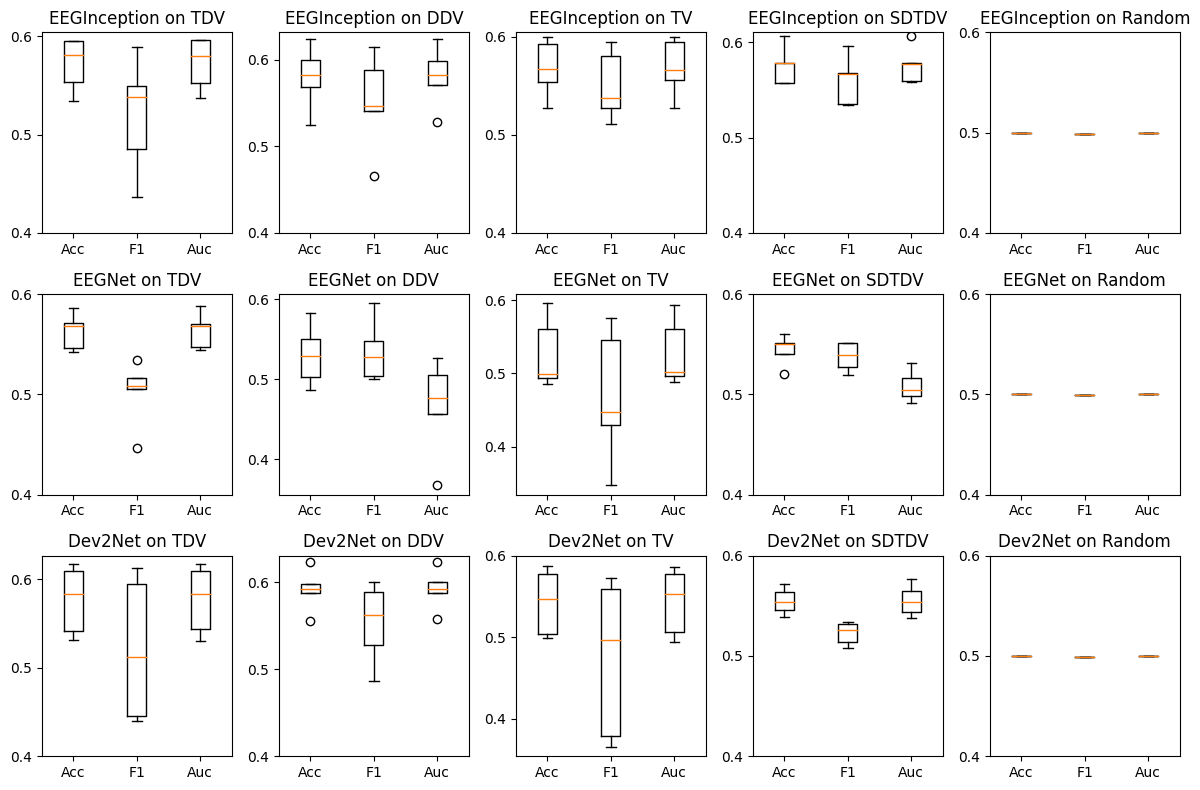
\includegraphics[width=\linewidth]{各日時各モデルごとの箱ひげ図.png}
    \caption{Each model for each validation}
    \label{fig: Each model for each validation}
\end{figure*}
\begin{figure*}[tb]
    \centering
    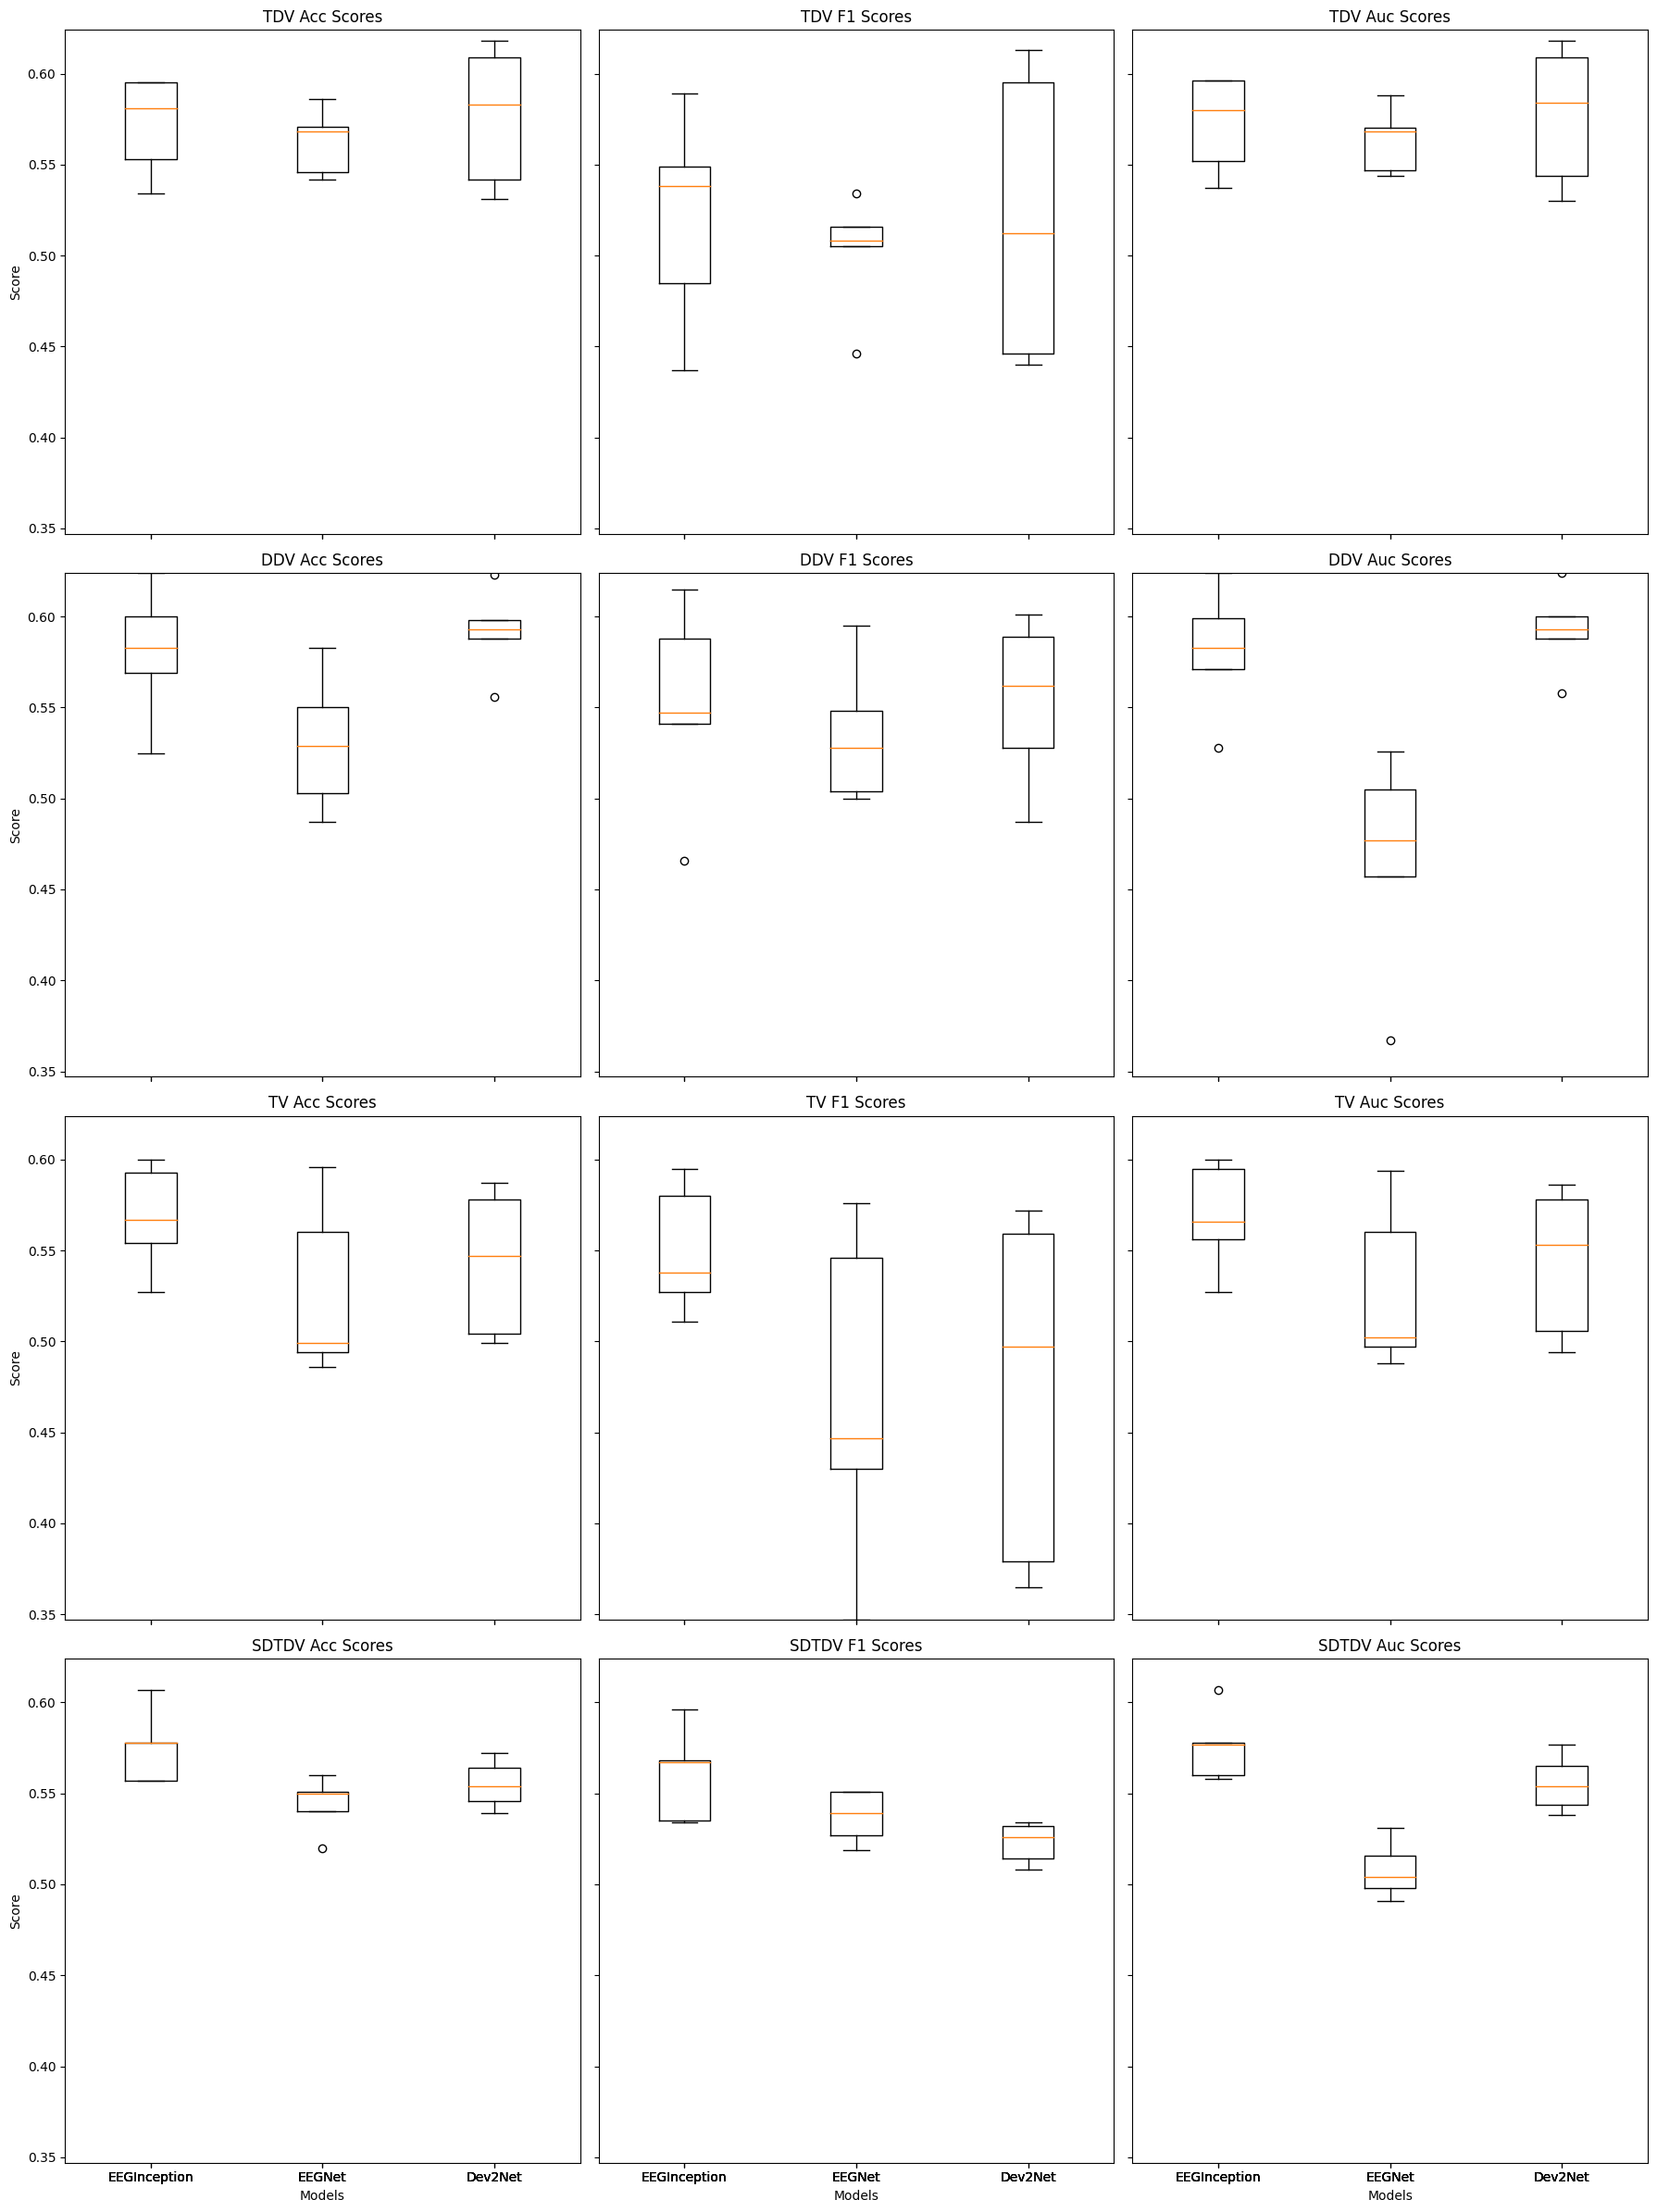
\includegraphics[width=\linewidth,height=0.95\textheight]{COMPARISON RESULTS FOR THE LEARNING CONDITION .png}
    \caption{Each evaluation for each validation.
    STDV has the lowest variance.
    TV has the largest variance.}
    \label{fig: Each evaluation  for each validation}
\end{figure*}
\begin{figure*}[tb]
    \centering
    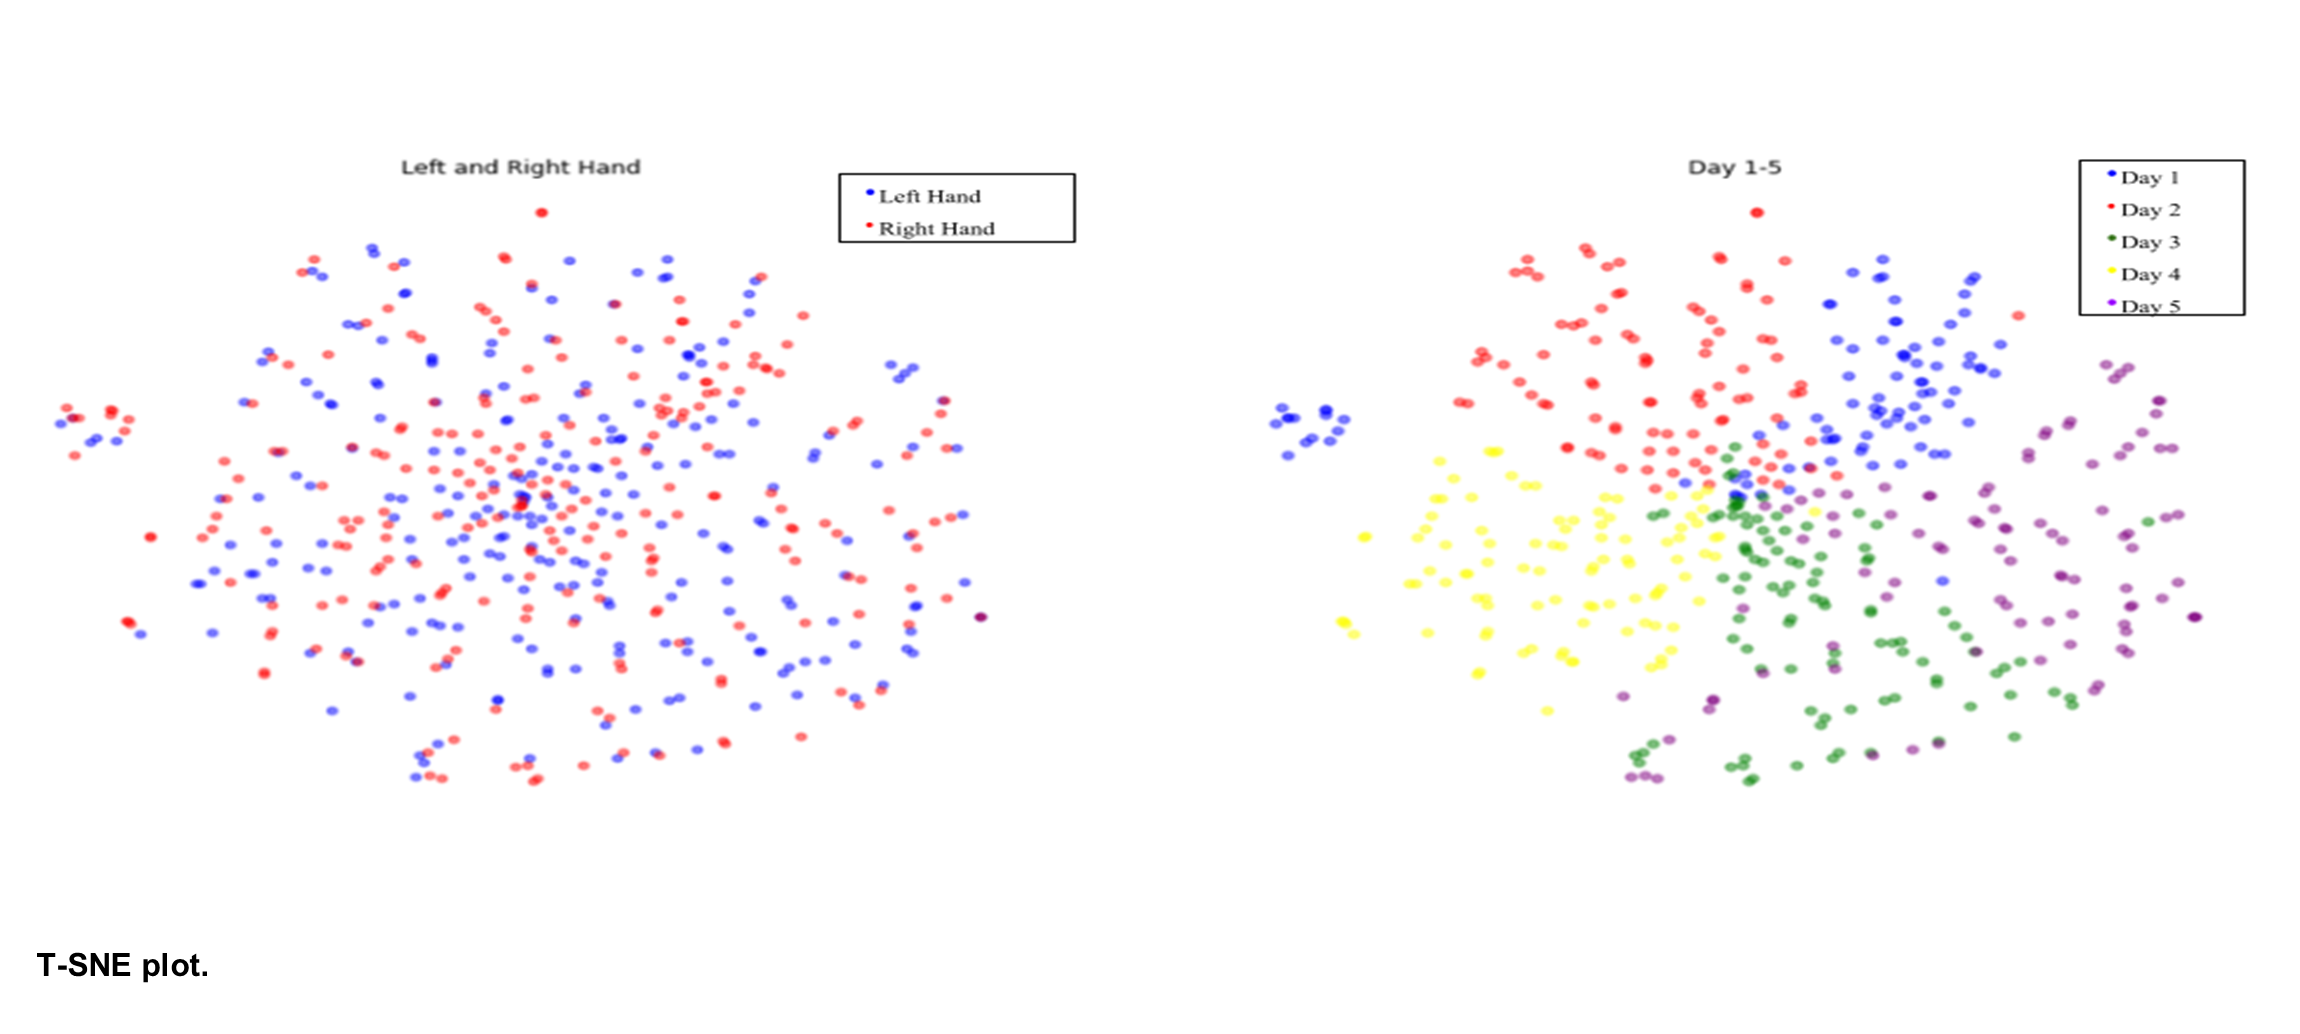
\includegraphics[width=1\linewidth]{画像12.png}
    \caption{T-SNE plot}
    \label{fig: T-SNE plot}
\end{figure*}

\begin{figure*}[tb]
    \centering
    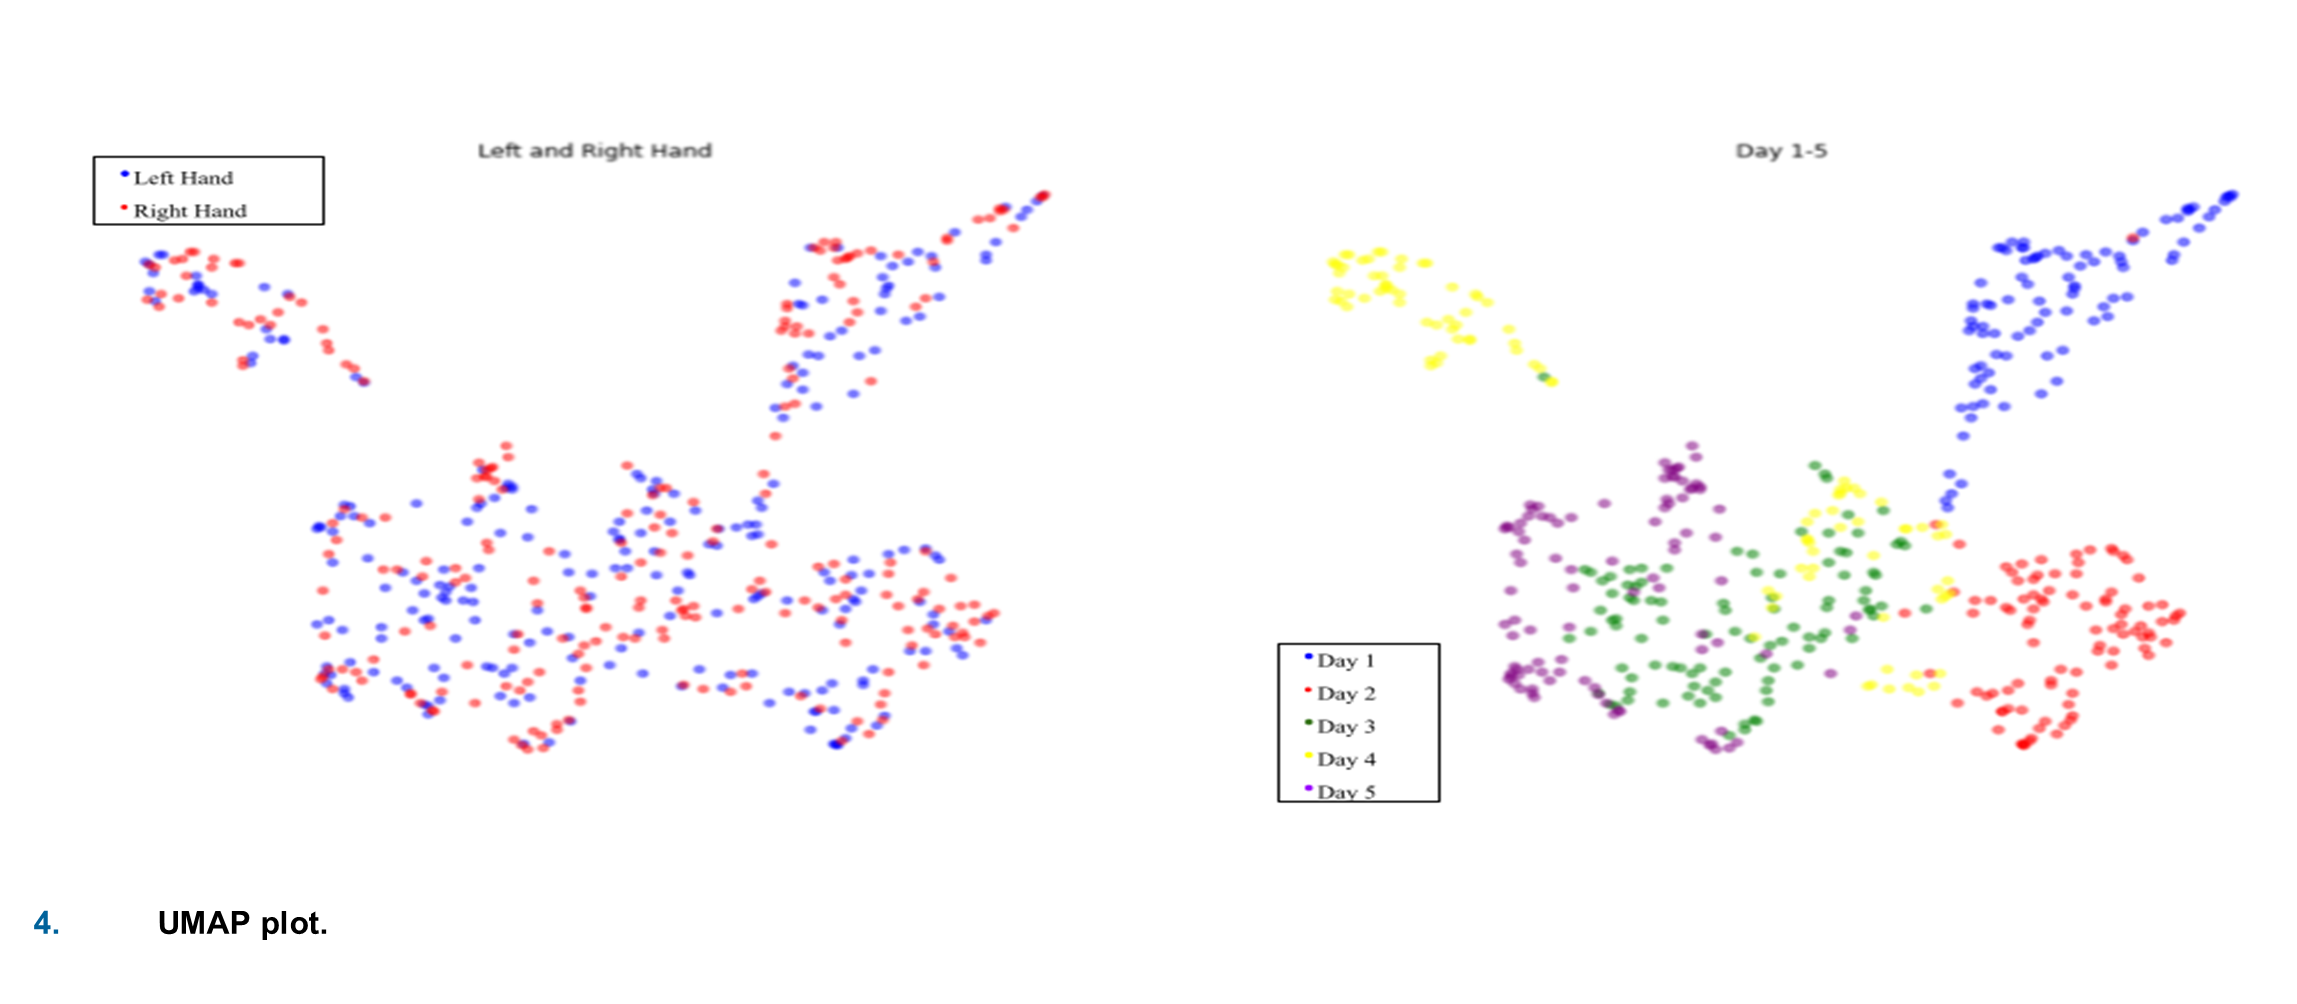
\includegraphics[width=1\linewidth]{画像13.png}
    \caption{UMAP plot}
    \label{fig: UMAP plot}
\end{figure*}

    \section{Evaluation of the Proposed Verification Techniques}
    \subsection{Performance evaluation metrics}
    The performance of each model was evaluated by its accuracy, F1-score, and AUC-ROC \cite{sharma2023recent}. These scores are used to evaluate the performance of the classification
    model. The term True Positive (TP) is used to describe the precise
    identification of a specific condition or trait, while False Positive (FP) describes
    the inaccurate identification of such a condition or trait. On the other
    hand, True Negative (TN) is used to describe the precise identification of the
    absence of a condition or trait, and False Negative (FN) indicates the
    inaccurate identification of this absence \cite{sharma2023recent}. These four classifications
    are fundamental in defining numerous performance measures.

    \subsubsection{Accuracy}
    Accuracy is the ratio of the number of correct predictions to the total number
    of predictions. It can be calculated.
    \begin{equation*}
        Accuracy=\frac{TP+TN}{TP+TN+FP+FN}\,. \tag{1}
    \label{equ:Acc}
    \end{equation*}

    \subsubsection{F1-score}
    The F1-score is the harmonic mean of precision and recall. It can be calculated.
    \begin{equation*}
        F1\text{score}= \frac{2 \times TP}{FN + FP + 2 \times TP}\,. \tag{2}
    \label{equ:F1}
    \end{equation*}

    \subsubsection{AUC}
    Receiver operating characteristics (ROC) is a curve plotted between true positive rate and false-positive rate. AUC is the area under this curve \cite{kuremoto2018enhancing}.


    \subsection{Performance Baseline}
    In each validation phase, labels were generated randomly via a binomial distribution
    and assessed using an evaluation index, comprising a precision of 0.5, an F1
    score of 0.5, and an AUC of 0.5. This is to establish criteria for model
    evaluation. Each model identifies motor recall (MI)-based 
    EEG for the subject's left and right hands. It is possible to identify
    models with poor performance when using randomly generated labels. Poor performance
    is indicated when the MI-based EEG data for the subject's left and right hands
    are captured inversely. For example, if the accuracy is 0.3 in the model-based
    evaluation, the accuracy in the binomial distribution is 0.5. In this case, the
    0.3 model captures the subject's left and right MI inversely. This is the
    criterion for the evaluation criterion to capture the generality of the
    model.
    \subsection{Bayesian ANOVA for Comparative Model Evaluation}
    A Bayesian analysis of variance (ANOVA)\cite{kruschke2010bayesian} is conducted, utilizing the mean
    accuracy derived from four distinct tests. This approach facilitates a comparative
    evaluation of the classification F1 scores across varying conditions. Such a
    statistical method is instrumental in discerning significant performance
    disparities among different models. Employing a variety of evaluation metrics
    and thorough statistical analyses enables a comprehensive assessment of model
    efficacy. Specifically, by scrutinizing F1 scores, one gains a profound
    understanding of each model's merits and limitations. Notably, Bayesian
    ANOVA is adept at pinpointing conditions that are conducive to enhanced
    classification accuracy, thereby aiding in the refinement of models and the development
    of more effective data collection protocols.

    \subsection{FLIPPED-LABEL DATASET COMPARISON}
    The labels are inverted when the model is trained on the MI-EEG of the
    subject's left and right hand movements. The purpose of this flipped-label dataset conparison is to
    compare the discrimination results of the generated model with those of the non-inverted
    model. Inverting the labels means, for example, that if a subject has a
    right-handed MI, he/she will be labeled with a left-handed MI. Once a
    correctly discriminating model is generated, the discrimination rate should be
    significantly reduced because the discrimination results are reversed when the
    left and right labels are inverted in the training data. If the
    identification rate is higher or the same as the baseline of the model, the method
    in question is not correctly generating a discriminative model. This is
    because the MI-EEG of the subject's left and right hand movements depends on
    the subject's way of thinking, and we want to verify whether the subject's MI-EEG
    is not causing the data to be unreproducible. In other words, we are trying to
    verify whether the MI-EEG data of the subject is reproducible even on multiple
    days, and whether the model is generalized.
    

\section{RESULT}
 
    \begin{table*}[tb]
        \centering
        \caption{Comparison of Variance Across Different Learning Conditions as Reflected in Table \ref{tab:COMPARISON RESULTS FOR THE LEARNING CONDITION}: A Detailed Analysis of Accuracies, F1 Scores, and AUC Metrics by Day and Model}
        \renewcommand{\arraystretch}{1.5}
        \resizebox{\linewidth}{3cm}{
        \begin{tabular}{|c|c|c|c|c|c|c|c|c|c|c|c|c|c|c|}
            \hline
            \multirow{2}{*}{Day} &\multirow{2}{*}{Evaluation} & \multicolumn{3}{c|}{TDV} & \multicolumn{3}{c|}{DDV} & \multicolumn{3}{c|}{TV} & \multicolumn{3}{c|}{SDTDV} & Random    \\
            \cline{3-15}
                        &            & EEG- Inception           & EEGNet                   & DevconvNet              & EEG- Inception             & EEGNet   & DevconvNet & EEG- Inception & EEGNet   & DevconvNet & EEG- Inception & EEGNet   & DevconvNet &          \\
            \hline
            \multirow{3}{*}{ Day 1} & Acc        & 7.25E-03                 & 9.21E-03                 & 9.21E-03                & 1.63E-02                   & 1.67E-03 & 1.35E-02   & 9.20E-03       & 5.04E-03 & 9.67E-04   & 1.10E-02       & 1.14E-02 & 1.04E-02   & 2.81E-07 \\
                                    & F1         & 1.71E-02                 & 1.99E-02                 & 1.99E-02                & 2.07E-02                   & 5.17E-03 & 2.24E-02   & 1.10E-02       & 7.80E-03 & 1.81E-01   & 1.37E-02       & 1.42E-02 & 1.47E-02   & 2.94E-07 \\
                                    & Auc        & 6.91E-03                 & 8.73E-03                 & 7.30E-02                & 6.20E-01                   & 1.46E-03 & 1.37E-02   & 9.21E-03       & 4.93E-03 & 5.17E-04   & 1.08E-02       & 1.17E+00 & 1.04E-02   & 2.83E-07 \\
            \hline
            \multirow{3}{*}{ Day 2} & Acc        & 1.24E-02                 & 1.50E-02                 & 4.40E-01                & 3.00E-01                   & 5.33E-03 & 1.89E-02   & 1.43E-02       & 7.09E-04 & 6.11E-04   & 1.27E-02       & 7.30E-03 & 6.07E-03   & 3.44E-07 \\
                                    & F1         & 2.06E-02                 & 2.34E-02                 & 1.47E-02                & 1.97E-02                   & 5.20E-03 & 3.05E-02   & 1.60E-02       & 1.73E-03 & 2.67E-03   & 1.43E-02       & 1.18E-02 & 9.40E-03   & 3.80E-07 \\
                                    & Auc        & 1.26E-02                 & 1.52E-02                 & 1.43E-02                & 1.81E-02                   & 5.29E-03 & 1.93E-02   & 1.43E-02       & 1.75E-04 & 6.68E-04   & 1.28E-02       & 7.36E-03 & 6.10E-03   & 3.43E-07 \\
            \hline
            \multirow{3}{*}{ Day 3} & Acc        & 1.26E-02                 & 8.19E-03                 & 7.86E-03                & 1.08E-02                   & 3.37E-03 & 2.27E-02   & 1.28E-02       & 1.60E-02 & 1.20E+00   & 1.29E-02       & 7.99E-03 & 1.04E-02   & 2.85E-07 \\
                                    & F1         & 1.99E-02                 & 1.02E-02                 & 1.59E-02                & 1.47E-02                   & 3.64E-03 & 2.41E-02   & 1.31E-02       & 1.92E-02 & 1.30E-02   & 1.45E-02       & 1.53E-02 & 1.30E-02   & 3.75E-07 \\
                                    & Auc        & 1.44E-02                 & 8.47E-03                 & 7.29E-03                & 1.01E-02                   & 3.09E-03 & 2.23E-02   & 1.29E-02       & 1.60E-02 & 1.19E-02   & 1.32E-02       & 7.93E-03 & 1.00E-02   & 2.79E-07 \\
            \hline
            \multirow{3}{*}{ Day 4} & Acc        & 1.68E-02                 & 1.40E-02                 & 1.78E-02                & 2.04E-02                   & 1.56E-03 & 2.22E-02   & 1.13E-02       & 2.99E-03 & 1.50E-03   & 2.18E-02       & 1.13E-02 & 1.70E-02   & 2.26E-07 \\
                                    & F1         & 2.49E-02                 & 1.71E-02                 & 3.09E-02                & 2.28E-02                   & 3.04E-03 & 2.64E-02   & 1.45E-02       & 6.26E-03 & 1.74E-02   & 2.45E-02       & 1.97E-02 & 2.50E-02   & 2.37E-07 \\
                                    & Auc        & 1.70E-02                 & 1.41E-02                 & 1.78E-02                & 2.03E-02                   & 1.37E-03 & 2.21E-02   & 1.13E-02       & 2.58E-03 & 1.47E-02   & 2.20E-02       & 1.14E-02 & 1.78E-02   & 2.26E-07 \\
            \hline
            \multirow{3}{*}{ Day 5} & Acc        & 1.77E-02                 & 1.32E-02                 & 1.80E-02                & 1.71E-02                   & 1.49E-02 & 2.06E-02   & 1.56E-02       & 1.70E-02 & 2.06E-02   & 1.57E-02       & 1.34E-02 & 1.70E-02   & 3.35E-07 \\
                                    & F1         & 1.85E-02                 & 2.55E-02                 & 2.02E-02                & 2.58E-02                   & 2.98E-02 & 2.67E-02   & 2.07E-02       & 1.90E-02 & 2.79E-02   & 1.95E-02       & 1.40E-02 & 2.70E-02   & 6.20E-07 \\
                                    & Auc        & 1.77E-02                 & 1.28E-02                 & 1.78E-02                & 1.72E-02                   & 1.45E-02 & 2.03E-02   & 1.50E-02       & 1.70E-02 & 1.98E-02   & 1.52E-02       & 1.34E-02 & 1.58E-02   & 3.40E-07 \\
            \hline
        \end{tabular}}

        \label{tab:VARIANCE COMPARISON}
    \end{table*}
    
    
  \begin{table*}[tb]
      \centering
      \caption{Comparison of methods using Bayesian analysis of variance for f1 scores.}
      \label{table:Comparison of methods using Bayesian analysis of variance for f1 scores.}
      \begin{tabular}{|l|r|r|r|r|r|r|r|r|}
          \hline
          Parameter        & SD     & hdi\_3\% & hdi\_97\% & mcse\_mean & mcse\_sd & ess\_bulk & ess\_tail & r\_hat \\
          \hline
          TDV means        & 0.520  & 0.014    & 0.495     & 0.545      & 0.0      & 0.0       & 5346.0    & 2678.0 \\
          \hline
          DDV means        & 0.551  & 0.014    & 0.526     & 0.577      & 0.0      & 0.0       & 4729.0    & 3310.0 \\
          \hline
          TV means         & 0.550  & 0.011    & 0.528     & 0.570      & 0.0      & 0.0       & 6730.0    & 3418.0 \\
          \hline
          SDTDV means      & 0.560  & 0.012    & 0.537     & 0.581      & 0.0      & 0.0       & 5050.0    & 3424.0 \\
          \hline
          TDV sigmas       & 0.151  & 0.010    & 0.132     & 0.169      & 0.0      & 0.0       & 5694.0    & 2888.0 \\
          \hline
          DDV sigmas       & 0.152  & 0.010    & 0.133     & 0.170      & 0.0      & 0.0       & 5054.0    & 3118.0 \\
          \hline
          TV sigmas        & 0.126  & 0.008    & 0.112     & 0.143      & 0.0      & 0.0       & 4897.0    & 2734.0 \\
          \hline
          SDTDV sigmas     & 0.133  & 0.008    & 0.118     & 0.149      & 0.0      & 0.0       & 4119.0    & 2925.0 \\
          \hline
          TDV diff\_means  & -0.026 & 0.012    & -0.048    & -0.004     & 0.0      & 0.0       & 5155.0    & 3023.0 \\
          \hline
          DDV diff\_means  & 0.006  & 0.012    & -0.016    & 0.027      & 0.0      & 0.0       & 4891.0    & 3131.0 \\
          \hline
          TV diff\_means   & 0.005  & 0.010    & -0.014    & 0.024      & 0.0      & 0.0       & 6416.0    & 3254.0 \\
          \hline
          SDTV diff\_means & 0.014  & 0.010    & -0.007    & 0.033      & 0.0      & 0.0       & 5120.0    & 3251.0 \\
          \hline
      \end{tabular} 
  \end{table*}
  
   \begin{table*}[tb]
    \centering
    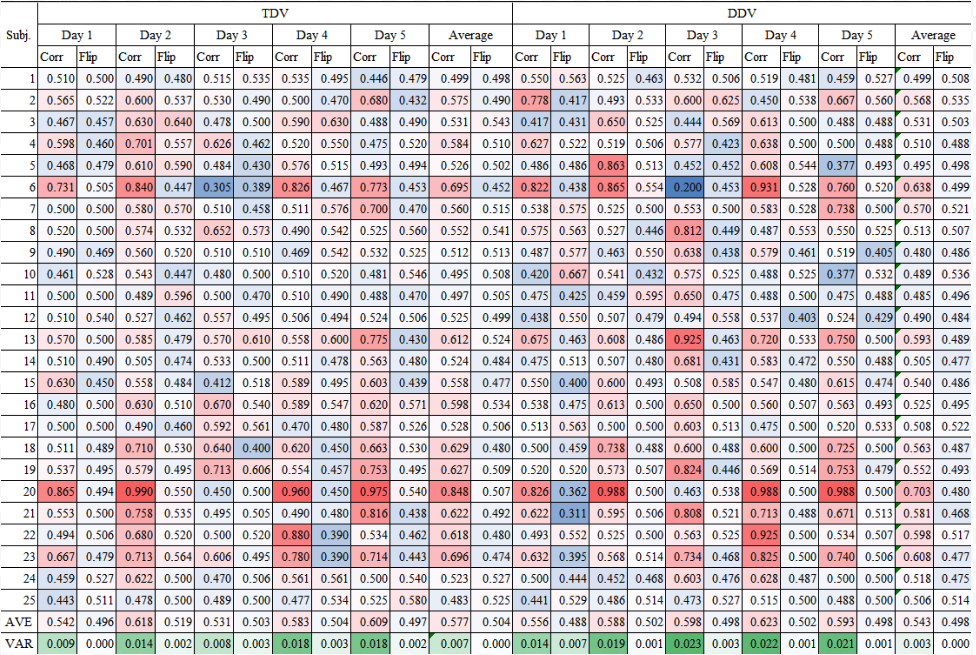
\includegraphics[width=\linewidth]{Flipdata.png}
    \caption{Learning with correct labels and learning with reversed labels for TDV and DDV EEGInception}
    \label{tab: Learning with correct labels and learning with reversed labels for TDV and DDV EEGInception}
    \end{table*}
    \subsection{Performance of the Proposed Verification Techniques}
    The analysis of TABLE\ref{tab:COMPARISON RESULTS FOR THE LEARNING CONDITION} offers a comprehensive understanding of the effectiveness of different learning conditions in EEG-based model training. The table compares five distinct approaches: TDV, DDV, TV, SDTDV, and a Random model across multiple metrics - Accuracy (Acc), F1-Score (F1), and Area Under Curve (Auc) - over a span of five days and an overall average.

    TDV approach shows moderate success. It consistently outperforms the Random model, suggesting the efficacy of pre-training on historical EEG data. However, when compared to other models, particularly DDV and SDTDV, its performance is not the most outstanding.
        
    DDV approach evident in its generally higher scores across all metrics, particularly on the fourth day. This suggests that including a small portion of test-day data can significantly boost the model's real-time identification accuracy. The highest numbers for ACC, F1-score, and AUC are colored pink.
        
    TV approach, which relies solely on test-day data, demonstrates a notable performance, especially in Accuracy and Auc metrics. This indicates that for certain applications, immediate day training without historical data might be sufficient, offering a more streamlined approach.
    
   SDTDV takes a more personalized approach, using only the subject's historical data for pre-training. This method's performance, particularly in Accuracy and F1-Score, is generally on par with TDV, indicating that individualized training does have merit, although it may not significantly outperform more generalized approaches.
    \vspace{1mm}
    \subsection{EEG Model Showdown: EEGInception Reigns Supreme}
    \vspace{1mm}
    Fig. \ref{fig: Each model for each validation}, \ref{fig: Each evaluation  for each validation} shows the classification accuracy (Acc), F1 score (F1), and area under the curve (AUC) are visualized. Boxplots are useful for showing the distribution, median, quartiles, and outliers of your data. The line in the middle of the box represents the median, the top and bottom edges of the box represent the third and first quartiles, respectively, and the whiskers are typically 1.5 times the interquartile range from the top and bottom quartiles. Indicates up to the outer data point. If a data point falls outside this range, it will be plotted as an outlier.
    
    
    \subsubsection{EEG Model Showdown: EEGInception Reigns Supreme}
    Key points discernible from Fig. \ref{fig: Each model for each validation} indicate that the performance of models across different validation sets is not consistent, and certain models may excel in specific validation sets. For instance, the Dev2Net model shows higher performance in the TDV and DDV validation sets but has smaller differences in others. On the other hand, EEGInception and EEGNet exhibit relatively stable performance, though not markedly superior in specific metrics or validation sets.
    
    \begin{itemize}
        \vspace{1mm}
      \item \textbf{EEGInception}: EEGInception model potentially exhibits a relatively narrow interquartile range, suggesting that the model provides consistent performance across various validation sets. It is expected to demonstrate stable performance, particularly on standardized datasets (TDV, DDV, TV), indicating EEGInception's adaptability to data with different characteristics and implying high generalization ability.
      \vspace{3mm}
      \item \textbf{EEGNet}: EEGNet model might show tendencies of wider interquartile ranges in specific validation sets, indicating sensitivity to specific data characteristics or significant performance variability under certain conditions. Performance instability in the DDV set could be anticipated, potentially reflecting the model's sensitivity to different data distributions. The breadth of EEGNet's interquartile range implies the necessity of caution in the model's adjustment or application.
      \vspace{3mm}
      \item \textbf{Dev2Net}: Dev2Net model demonstrates good performance in TDV and DDV sets, the possibility of wider interquartile ranges compared to other models suggests potential significant performance variability under some conditions. This might indicate that Dev2Net can achieve high performance but is strongly dependent on the characteristics of specific datasets. Significant variability in metrics like F1 score or AUC could reflect the model's sensitivity to the balance between different classes or the identification of specific classes.
    \end{itemize}


    \subsubsection{Dependency of Model Performance on Validation Method}

    From Fig. \ref{fig: Each evaluation  for each validation}, it is evident that there is a significant difference in the distribution of scores across various validation methods and models, indicating that model performance is contingent upon the validation method employed. Some models demonstrate high accuracy, F1 scores, and AUC in certain validation methods while underperforming in others, highlighting the influence of validation methodologies on model efficacy. The consistency of scores in Random validation (around 0.5) suggests its role as a baseline.

    Fluctuation in model performance across different validation methods may suggest that certain models are more apt for specific types of data or problem configurations. For instance, the EEGInception model consistently outperforms others in TDV and DDV validations but not in TV validation, suggesting its enhanced capability to capture certain data characteristics or its effective regularization against overfitting in specific contexts. Conversely, the Dev2Net model exhibits stable performance in TDV and DDV, occasionally surpassing other models in AUC, indicating its potential superior generalizability across diverse datasets and problem settings.
    \begin{itemize}
        \vspace{1mm}
        \item \textbf{TDV}: Relatively wide interquartile range (IQR) observed for the Dev2Net model in TDV might indicate its high adaptability to training data without directly translating to consistent performance improvement. In contrast, a narrower IQR for the EEGInception model implies its stable performance on training data.
        \vspace{3mm}
        \item \textbf{DDV}: In DDV, the IQR, especially for the EEGInception and Dev2Net models, reflects their capability to adapt to different data characteristics. A narrow IQR for EEGInception suggests its ability to maintain stable performance across various datasets, while a wide IQR for Dev2Net indicates potential performance variability.
        \vspace{3mm}
        \item \textbf{TV}: Breadth of the IQR in TV validation acts as an indicator of a model's generalization ability to test data, where a wider IQR suggests potential instability in performance on unfamiliar data. This is particularly relevant for the EEGNet model, which may show considerable performance variability across different testing scenarios.
        \vspace{3mm}
        \item \textbf{SDTDV}: Validation through SDTDV is advantageous for minimizing accuracy variance. The analysis of the IQR in SDTDV allows for the assessment of a model's adaptability to semi-diverse training data. A narrow IQR indicates that a model consistently performs well on such data. EEGInception and Dev2Net displaying a relatively narrow IQR suggests their capability to maintain stable performance across semi-diverse datasets.
    \end{itemize}
    \vspace{1mm}
    
    \subsection{Daily variations in learning conditions and comparisons between models in EEG analysis }
    Table \ref{tab:VARIANCE COMPARISON} summarises the analysis of EEG data under different learning conditions. Several EEG analysis models, including EEG-Inception, EEGNet, and DevconvNet, were used to assess the variability of subjects' performance.

    Table \ref{tab:VARIANCE COMPARISON} presents the values of 'Acc (Accuracy)', 'F1 (F1 score)', and 'Auc (area under the curve)' for each day, indicating considerable variability in model performance from day to day. It is important to note that certain models have different accuracy and F1 scores between 'Day 1' and 'Day 3', indicating that training conditions and subject responses may vary day to day.
    
    When comparing different models, each one performs better on specific assessment measures. 'EEG-Inception' and 'DevconvNet' have higher 'Auc' values on some days, suggesting that these models may have better discriminative ability under certain conditions.
    
    
    \subsection{Comparison of methods by Bayesian analysis of variance}
    Table \ref{table:Comparison of methods using Bayesian analysis of variance for f1 scores.} compares four methods: TDV, DDV, TV, and SDTDV, using Bayesian analysis of variance. The means of each method are 0.520, 0.551, 0.550, and 0.560, respectively, with SDTDV having the highest mean value. However, this difference is not significant compared to the other methods. It is important to note that all methods have similar means and should be considered equally effective. Therefore, this result suggests that SDTDV is not significantly superior to the other methods.

    A comparison of standard deviations was conducted. The standard deviations for TDV, DDV, TV and SDTDV are 0.151, 0.152, 0.126 and 0.133 respectively. This shows that TV has the lowest standard deviation, indicating that it is more consistent in its results than the other methods.

    The mean difference between the methods reveals that TDV has the smallest difference at -0.026. DDV, TV, and SDTDV have differences close to zero, suggesting that their means are similar. This result indicates that all methods perform similarly.

     Additionally, we examine the ESS and r\_hat values, which serve as indicators of the quality of Bayesian analysis. The high ESS values and r\_hat values close to 1 for all methods indicate good model convergence. The analysis results are highly reliable.

    TV shows the best results compared to other methods, with the lowest standard deviation indicating high consistency. However, the other methods also have small performance differences, so it is important to select the appropriate method depending on the purpose and situation. The analysis is highly reliable, as evidenced by the high ESS values and r\_hat values close to 1 obtained for all methods.
    \subsection{Some subjects are more accurate when labels are reversed}
    Table \ref{tab: Learning with correct labels and learning with reversed labels for TDV and DDV EEGInception} compares learning with correct labels and learning with reversed labels for TDV and DDV EEGInception, by day of the week and by subject. The desired result of inverted-labels learning should be a recognition result of less than 50\% in almost all cases, but in reality, identification is performed with an average of 50\% and microscopic variation. As the labels are learnt by inverting the labels, this would normally have to be below the accuracy of normal learning in all subjects. Some subjects tend to show an average of 53\% agreement over a five-day period, even when learning opposite labels. Some have exceeded the accuracy of learning the labels inverted. This phenomenon suggests that some subjects may be presenting opposite signals based on the general EEG tendencies of other subjects.
    \begin{table*}
        \centering
        \caption{Comparison of existing and proposed methods in this study}
        \begin{tabularx}{\linewidth}{|X|X|X|X|X|X|X|}
            \hline
            Method & Number of Subjects & Number of Days & Algorithm & Feature Extraction & Objective & Publicly Available? \tabularnewline \hline
            Amjad Abu-Rmileh method\cite{kaya2023identifying} & 18 & 4 days & LDA Classifier based on Subject-Specific $\alpha$, $\beta$ Frequency Bands & Yes (EEG Power Spectrum based on $\alpha$, $\beta$ Frequency Bands) & Improving the Effectiveness of EEG-Based BCI Training Using an Adaptive LDA Classifier & No \tabularnewline \hline
            Esra Kaya method\cite{abu2019co} & 1 & 20 days & Ensemble Subspace Discriminant Classifier & Yes (Time, Frequency, Spatiotemporal, Nonlinear Features) & Finding the Optimal Channel & No \tabularnewline \hline
            ma2022\cite{ma2022large} & 25 & 5 days & Common Spatial Patterns (CSP), Filter Bank Common Spatial Pattern (FBCSP), Filter-bank Convolutional Network (FBCNet), EEGNet, Deep Convolutional Network (deep ConvNets), Adaptive Transfer Learning & Yes (Using algorithms such as CSP, FBCSP) & Improving Cross-Session Classification in Brain-Computer Interfaces (BCI) using Motor Imagery (MI) & Yes (Open Access Dataset) \tabularnewline \hline
            our Method & 25 & 5 days & Convolutional Network, Transformer, Graph Network & No & Reproducibility Verification in BCI using Motor Imagery (MI) & Yes (Open Access Dataset) \tabularnewline \hline
        \end{tabularx}
        \label{tab: Comparison of existing and proposed methods in this study}
    \end{table*}
    
\section{Discussion}
    
    The comprehensive analysis presented in the results offers several key insights into the effectiveness of different learning approaches for EEG-based model training. 
    
    First, it is evident that utilizing historical EEG data to pre-train models, as done in the TDV approach, leads to moderate performance improvements over a random baseline. This confirms the utility of leveraging the existing subject data to initialize model parameters before fine-tuning new unseen data. However, TDV is outperformed by approaches that incorporate same-day data.
    
    In particular, the DDV technique, which supplements pre-training data with a small portion of test-day data for fine-tuning, demonstrates superior overall performance. Across all days and metrics, DDV achieves higher scores compared to solely relying on historical data. This highlights the benefits of adaptivity by allowing models to fine-tune current test data characteristics. As a result, significant boosts in real-time EEG decoding accuracy can be attained.
    
    Interestingly, the results also showcase the viability of a purely test-day-based approach with the TV method. Despite lacking any historical data, TV displays competitive performance, even occasionally outperforming techniques like TDV that utilize past subject data. This indicates that for certain real-time applications, historical data may not be an absolute prerequisite, thereby enabling more streamlined deployments.
    
    Additionally, the analysis also sheds light on the utility of personalized model training. The SDTDV technique, which trains exclusively on individual subject history, largely keeps pace with more generalized approaches like TDV, in terms of accuracy and F1 scores. This underscores the importance of accounting for inter-subject variability in EEG patterns through individualized calibration. However, SDTDV does not definitively outperform other methods, suggesting the need for more research into personalized adaptive systems.
    
    
    The variability in the performance of the assessed EEG analysis models (Fig. \ref{fig: Each evaluation for each validation}) further highlights the interaction effects between datasets and algorithms. Selecting the optimal approach is contingent on the task specifications and data characteristics. Adaptive methods like DDV could be preferential for applications requiring real-time EEG decoding under changing conditions. Meanwhile, robust generalized techniques like EEGInception may be better suited for offline analysis tasks.
    
    Overall, the findings strongly advocate for increased incorporation of adaptivity in EEG analysis systems, either via fine-tuning current data or reliance on test-day statistics. Pre-training on subject history still holds merit, but must be augmented with calibration on fresh same-day data to maximize decoding accuracies. There also remains promise in personalized adaptive systems that account for inter-subject variability. Furthermore, the optimal algorithm is dependent on the intended real-time or offline use case specifications.
    
    A key limitation of the current analysis is the reliance on a single publicly available dataset, restricting conclusion generalizability. Further validation on diverse private clinical and research EEG data repositories could strengthen these insights and provide greater confidence in the superiority of adaptive learning schemes. Additionally, more methodical hyperparameter optimization and neural architecture searches could help boost model performances. In the future, promising research directions include the development of unified adaptive frameworks that enable seamless integration of multiday historical and real-time daily data for optimized subject-specific EEG analysis.

    
    The T-SNE\cite{van2008visualizing} and UMAP\cite{sainburg2021parametric}(Fig. \ref{fig: T-SNE plot}, \ref{fig: UMAP plot}) visualizations offer insight into the model's ability to discriminate between subjects using EEG data across multiple days. A key observation is that when labels and days are encoded (right plots), some separation is visible between data points from different days. This indicates that the model has learned features related to day-specific variability in the EEG data.

    However, in the label-only plots (left plots), the data points are largely mixed without clear separation between the classes. This suggests that the model struggles to extract discriminative features for identifying individuals, irrespective of the day. The lack of inter-subject variability encoding is a major weakness.
    
    A likely explanation is that due to fluctuations in EEG signals across days, the model primarily learns features associated with daily variability rather than subject-specific trait-based patterns. This is aligned with past research showing within-person EEG fluctuations across time.
    
    The analysis has significant implications regarding model optimization for EEG-based identification. For instance, the poor subject discrimination performance highlights the need for more reliable trait-based biomarkers that are consistent across sessions. Additionally, the prominence of day-specific patterns indicates that longitudinal calibration may be necessary through sequential fine-tuning approaches.
    
    The coverage limitations of SDTDV models trained on individual subject data likely contribute to the lack of a consistent view of the target feature space across days. Broader TDV or DDV approaches could help mitigate this issue. However, the possibility of divergence between the pretrained and test spaces remains a risk.
    
    In summary, the observations emphasize the complex interactions between the intra-subject longitudinal variability and inter-subject trait-based patterns in EEG signals. Enhancing model robustness likely requires a hybrid approach of extracting reliable identifying biomarkers while accounting for cyclical fluctuations through adaptive calibration. This could pave the path toward translating EEG-based biometrics from controlled scenarios to more practical free-living applications.
    
    \section{Conclusion}
This research aimed to validate the reproducibility of MI-based EEG datasets and the universality of the discrimination algorithms used. The extensive multi-day MI-EEG dataset with 25 participants enabled the analysis of EEG signal consistency over time. Four EEG verification techniques were compared through experiments, namely, TDV, DDV, TV, and SDTDV. Results demonstrated that incorporating a small portion of test day data for model adaptation (as in DDV) yielded higher accuracy than solely relying on pre-training data (TDV). This highlights the potential of adaptive, real time learning models that account for intra-subject variability in EEG patterns. Meanwhile, the competitive performance of TV indicates that in certain applications, test day training alone may suffice over pre-training approaches. The similarity in outcomes between generalized (TDV) and personalized (SDTDV) training suggests that while individual differences exist in EEG data, generalized models can prove effective for MI classification tasks. Overall, the study verifies the reproducibility of MI-EEG signals over multiple days and the viability of using generalized discrimination algorithms. This research pioneers a pragmatic approach to evaluating the real-world effectiveness of MI-EEG systems beyond laboratory conditions. The methodology and findings pave the way for more adaptive, subject-specific, instantly calibrated EEG interfaces. By demonstrating robust reproducibility and model generalizability, this study marks an important step toward transitioning MI-EEG technology into practical assistive and therapeutic applications. An area for future work is investigating reproducibility over more extended durations spanning months or years.
    \begin{landscape}
        \centering
        \begin{table}[tb]
          \caption{ACCURACY COMPARISON BETWEEN SUBJECTS IN THE DECONVNET RESULTS}
          \label{table:ACCURACY COMPARISON BETWEEN SUBJECTS IN THE DECONVNET RESULTS} 
          \small
          \resizebox{\columnwidth}{!}{%
          \begin{tabular}{|c|c|c|c|c|c|c|c|c|c|c|c|c|c|c|c|c|c|c|c|c|c|c|c|c|}
              \hline
                    & \multicolumn{6}{|c|}{TDV} & \multicolumn{6}{|c|}{DDV} & \multicolumn{6}{|c|}{TV} & \multicolumn{6}{|c|}{SDTDV} \\
              \hline
              Subj. & Day 1                     & Day 2                     & Day 3                    & Day 4                      & Day 5 & AVE   & Day 1 & Day 2 & Day 3 & Day 4 & Day 5 & AVE   & Day 1 & Day 2 & Day 3 & Day 4 & Day 5 & AVE   & Day 1 & Day 2 & Day 3 & Day 4 & Day 5 & AVE   \\
              \hline
              1     & 0.51                      & 0.49                      & 0.515                    & 0.535                      & 0.446 & 0.499 & 0.55  & 0.525 & 0.532 & 0.519 & 0.459 & 0.517 & 0.425 & 0.513 & 0.582 & 0.468 & 0.446 & 0.487 & 0.53  & 0.56  & 0.434 & 0.455 & 0.568 & 0.509 \\
              \hline
              2     & 0.565                     & 0.6                       & 0.53                     & 0.5                        & 0.68  & 0.575 & 0.778 & 0.493 & 0.6   & 0.45  & 0.667 & 0.598 & 0.514 & 0.453 & 0.488 & 0.488 & 0.533 & 0.495 & 0.533 & 0.547 & 0.52  & 0.5   & 0.587 & 0.537 \\
              \hline
              3     & 0.467                     & 0.63                      & 0.478                    & 0.59                       & 0.488 & 0.531 & 0.417 & 0.65  & 0.444 & 0.613 & 0.488 & 0.522 & 0.542 & 0.55  & 0.458 & 0.513 & 0.538 & 0.52  & 0.5   & 0.54  & 0.576 & 0.5   & 0.525 & 0.528 \\
              \hline
              4     & 0.598                     & 0.701                     & 0.626                    & 0.52                       & 0.475 & 0.584 & 0.627 & 0.519 & 0.577 & 0.638 & 0.5   & 0.572 & 0.507 & 0.532 & 0.648 & 0.563 & 0.613 & 0.573 & 0.54  & 0.474 & 0.549 & 0.49  & 0.488 & 0.508 \\
              \hline
              5     & 0.468                     & 0.61                      & 0.484                    & 0.576                      & 0.493 & 0.526 & 0.486 & 0.863 & 0.452 & 0.608 & 0.377 & 0.557 & 0.514 & 0.475 & 0.575 & 0.506 & 0.478 & 0.51  & 0.564 & 0.52  & 0.559 & 0.515 & 0.478 & 0.527 \\
              \hline
              6     & 0.731                     & 0.84                      & 0.305                    & 0.826                      & 0.773 & 0.695 & 0.822 & 0.865 & 0.2   & 0.931 & 0.76  & 0.715 & 0.466 & 0.527 & 0.533 & 0.639 & 0.587 & 0.55  & 0.559 & 0.702 & 0.411 & 0.522 & 0.467 & 0.532 \\
              \hline
              7     & 0.5                       & 0.58                      & 0.51                     & 0.511                      & 0.7   & 0.56  & 0.538 & 0.525 & 0.553 & 0.583 & 0.738 & 0.587 & 0.488 & 0.5   & 0.526 & 0.625 & 0.425 & 0.513 & 0.61  & 0.49  & 0.552 & 0.554 & 0.475 & 0.536 \\
              \hline
              8     & 0.52                      & 0.574                     & 0.652                    & 0.49                       & 0.525 & 0.552 & 0.575 & 0.527 & 0.812 & 0.487 & 0.55  & 0.59  & 0.513 & 0.514 & 0.768 & 0.5   & 0.438 & 0.546 & 0.5   & 0.415 & 0.506 & 0.5   & 0.488 & 0.482 \\
              \hline
              9     & 0.49                      & 0.56                      & 0.51                     & 0.469                      & 0.532 & 0.512 & 0.487 & 0.463 & 0.638 & 0.579 & 0.519 & 0.537 & 0.474 & 0.463 & 0.588 & 0.513 & 0.43  & 0.494 & 0.49  & 0.49  & 0.48  & 0.427 & 0.456 & 0.469 \\
              \hline
              10    & 0.461                     & 0.543                     & 0.48                     & 0.51                       & 0.481 & 0.495 & 0.42  & 0.541 & 0.575 & 0.488 & 0.377 & 0.48  & 0.551 & 0.527 & 0.65  & 0.563 & 0.455 & 0.549 & 0.416 & 0.574 & 0.49  & 0.54  & 0.519 & 0.508 \\
              \hline
              11    & 0.5                       & 0.489                     & 0.5                      & 0.51                       & 0.488 & 0.497 & 0.475 & 0.459 & 0.65  & 0.488 & 0.475 & 0.509 & 0.525 & 0.486 & 0.688 & 0.5   & 0.488 & 0.537 & 0.47  & 0.479 & 0.4   & 0.47  & 0.525 & 0.469 \\
              \hline
              12    & 0.51                      & 0.527                     & 0.557                    & 0.506                      & 0.524 & 0.525 & 0.438 & 0.507 & 0.494 & 0.537 & 0.524 & 0.5   & 0.45  & 0.507 & 0.468 & 0.463 & 0.413 & 0.46  & 0.52  & 0.571 & 0.454 & 0.529 & 0.413 & 0.497 \\
              \hline
              13    & 0.57                      & 0.585                     & 0.57                     & 0.558                      & 0.775 & 0.612 & 0.675 & 0.608 & 0.925 & 0.72  & 0.75  & 0.736 & 0.463 & 0.527 & 0.913 & 0.653 & 0.938 & 0.699 & 0.7   & 0.5   & 0.82  & 0.579 & 0.825 & 0.685 \\
              \hline
              14    & 0.51                      & 0.505                     & 0.533                    & 0.511                      & 0.563 & 0.524 & 0.475 & 0.507 & 0.681 & 0.583 & 0.55  & 0.559 & 0.525 & 0.52  & 0.639 & 0.486 & 0.575 & 0.549 & 0.53  & 0.505 & 0.522 & 0.543 & 0.638 & 0.548 \\
              \hline
              15    & 0.63                      & 0.558                     & 0.412                    & 0.589                      & 0.603 & 0.558 & 0.55  & 0.6   & 0.508 & 0.547 & 0.615 & 0.564 & 0.513 & 0.52  & 0.385 & 0.507 & 0.5   & 0.485 & 0.49  & 0.653 & 0.471 & 0.726 & 0.487 & 0.565 \\
              \hline
              16    & 0.48                      & 0.63                      & 0.67                     & 0.589                      & 0.62  & 0.598 & 0.538 & 0.613 & 0.65  & 0.56  & 0.563 & 0.585 & 0.5   & 0.5   & 0.675 & 0.533 & 0.521 & 0.546 & 0.61  & 0.56  & 0.64  & 0.568 & 0.451 & 0.566 \\
              \hline
              17    & 0.5                       & 0.49                      & 0.592                    & 0.47                       & 0.587 & 0.528 & 0.513 & 0.5   & 0.603 & 0.475 & 0.52  & 0.522 & 0.5   & 0.488 & 0.59  & 0.625 & 0.48  & 0.536 & 0.47  & 0.53  & 0.51  & 0.47  & 0.613 & 0.519 \\
              \hline
              18    & 0.511                     & 0.71                      & 0.64                     & 0.62                       & 0.663 & 0.629 & 0.5   & 0.738 & 0.6   & 0.6   & 0.725 & 0.633 & 0.446 & 0.45  & 0.613 & 0.588 & 0.513 & 0.522 & 0.426 & 0.58  & 0.67  & 0.49  & 0.55  & 0.543 \\
              \hline
              19    & 0.537                     & 0.579                     & 0.713                    & 0.554                      & 0.753 & 0.627 & 0.52  & 0.573 & 0.824 & 0.569 & 0.753 & 0.648 & 0.547 & 0.507 & 0.595 & 0.556 & 0.452 & 0.531 & 0.505 & 0.537 & 0.553 & 0.522 & 0.616 & 0.547 \\
              \hline
              20    & 0.865                     & 0.99                      & 0.45                     & 0.96                       & 0.975 & 0.848 & 0.826 & 0.988 & 0.463 & 0.988 & 0.988 & 0.85  & 0.493 & 0.513 & 0.5   & 0.963 & 1     & 0.694 & 0.843 & 0.67  & 0.47  & 0.99  & 0.925 & 0.78  \\
              \hline
              21    & 0.553                     & 0.758                     & 0.495                    & 0.49                       & 0.816 & 0.622 & 0.622 & 0.595 & 0.808 & 0.713 & 0.671 & 0.682 & 0.5   & 0.519 & 0.685 & 0.688 & 0.658 & 0.61  & 0.777 & 0.616 & 0.699 & 0.67  & 0.816 & 0.715 \\
              \hline
              22    & 0.494                     & 0.68                      & 0.5                      & 0.88                       & 0.534 & 0.618 & 0.493 & 0.525 & 0.563 & 0.925 & 0.534 & 0.608 & 0.507 & 0.5   & 0.525 & 0.863 & 0.575 & 0.594 & 0.471 & 0.73  & 0.52  & 0.75  & 0.534 & 0.601 \\
              \hline
              23    & 0.667                     & 0.713                     & 0.606                    & 0.78                       & 0.714 & 0.696 & 0.632 & 0.568 & 0.734 & 0.825 & 0.74  & 0.7   & 0.5   & 0.5   & 0.532 & 0.688 & 0.597 & 0.563 & 0.615 & 0.638 & 0.707 & 0.83  & 0.766 & 0.711 \\
              \hline
              24    & 0.459                     & 0.622                     & 0.47                     & 0.561                      & 0.5   & 0.523 & 0.5   & 0.452 & 0.603 & 0.628 & 0.5   & 0.537 & 0.5   & 0.516 & 0.556 & 0.487 & 0.45  & 0.502 & 0.459 & 0.488 & 0.542 & 0.551 & 0.575 & 0.523 \\
              \hline
              25    & 0.443                     & 0.478                     & 0.489                    & 0.477                      & 0.525 & 0.483 & 0.441 & 0.486 & 0.473 & 0.515 & 0.488 & 0.48  & 0.515 & 0.486 & 0.5   & 0.485 & 0.575 & 0.512 & 0.511 & 0.478 & 0.415 & 0.409 & 0.513 & 0.465 \\
              \hline
              AVE   & 0.542                     & 0.618                     & 0.531                    & 0.583                      & 0.609 & 0.577 & 0.556 & 0.588 & 0.598 & 0.623 & 0.593 & 0.592 & 0.499 & 0.504 & 0.587 & 0.578 & 0.547 & 0.543 & 0.546 & 0.554 & 0.539 & 0.564 & 0.572 & 0.555 \\
              \hline
              VAR   & 0.009                     & 0.014                     & 0.008                    & 0.018                      & 0.018 & 0.007 & 0.014 & 0.019 & 0.023 & 0.022 & 0.021 & 0.008 & 0.001 & 0.001 & 0.012 & 0.015 & 0.021 & 0.003 & 0.01  & 0.006 & 0.01  & 0.018 & 0.017 & 0.007 \\
              \hline
          \end{tabular}%
          }
      \end{table}
    \end{landscape}
    \begin{landscape}
    \begin{table}[tb]
        \caption{Comparison of existing data sets and the data sets used in this study}
        \begin{tabularx}{\linewidth}{|p{2.5cm}|X|X|X|X|X|X|X|X|X|}
        \hline
        \textbf{Dataset} & \textbf{\#Subj} & \textbf{\#Chan} & \textbf{\#Classes} & \textbf{\#Trials} & \textbf{Trial length} & \textbf{Freq} & \textbf{BCI} & \textbf{Multiple days} & \textbf{EOG Acquisition} \\ \hline
        AlexMI\cite{alexandre2006commande} & 8 & 16 & 3 & 20 & 3s & 512Hz & g.USBamp & No (Details Unknown) & No \\ \hline
        BNCI2014\_001\cite{tangermann2012review} & 9 & 22 & 4 & 144 & 4s & 250Hz & Not & Yes (2 days) & Yes \\ \hline
        BNCI2014\_002\cite{steyrl2016random} & 14 & 15 & 2 & 80 & 5s & 512Hz & g.USBamp & No & No \\ \hline
        BNCI2014\_004\cite{leeb2007brain} & 9 & 3 & 2 & 360 & 4.5s & 250Hz & g.tec & Yes (2 days) & Yes \\ \hline
        BNCI2015\_001\cite{faller2012autocalibration} & 12 & 13 & 2 & 200 & 5s & 512Hz & g.GAMMAsys & No & No \\ \hline
        BNCI2015\_004\cite{scherer2015individually} & 9 & 30 & 5 & 80 & 7s & 256Hz & g.tec GAMMAsys system & Yes (2 days) & No \\ \hline
        Cho2017\cite{cho2017eeg} & 52 & 64 & 2 & 100 & 3s & 512Hz & Biosemi ActiveTwo system & No & Yes \\ \hline
        GrosseWentrup2009\cite{grosse2009beamforming} & 10 & 128 & 2 & 150 & 7s & 500Hz & Not specified & No & Yes \\ \hline
        Lee2019\_MI\cite{lee2019eeg} & 54 & 62 & 2 & 100 & 4s & 1000Hz & BrainAmp & No & No \\ \hline
        Ofner2017\cite{ofner2017upper} & 15 & 61 & 7 & 60 & 3s & 512Hz & g.tec & Yes (2 days) & No \\ \hline
        PhysionetMI\cite{schalk2004bci2000} & 109 & 64 & 4 & 23 & 3s & 160Hz & Not specified & No & No \\ \hline
        Schirrmeister2017\cite{schirrmeister2017deep} & 14 & 128 & 4 & 120 & 4s & 500Hz & Not specified & No & No \\ \hline
        Shin2017A\cite{shin2016open} & 29 & 30 & 2 & 30 & 10s & 200Hz & BrainAmp & No & Yes \\ \hline
        Shin2017B\cite{shin2016open} & 29 & 30 & 2 & 30 & 10s & 200Hz & BrainAmp & No & Yes \\ \hline
        Weibo2014\cite{yi2014evaluation} & 10 & 60 & 7 & 80 & 4s & 200Hz & Neuroscan SynAmps2 & No & Yes \\ \hline
        Zhou2016\cite{zhou2016fully} & 4 & 14 & 3 & 160 & 5s & 250Hz & Not specified & Yes (3 days) & No \\ \hline
        dreyer2023\cite{dreyer2023large} & 87 & 27 & 2 & 40 & 8s & 512Hz & g.USBAmp & No & Yes \\ \hline
        \rowcolor{pink} ma2022\cite{ma2022large} & 25 & 32 & 2 & 90-100 & 7.5s & 250Hz & Wuhan Greentech Technology Co. LTD & Yes(5days) & No \\ \hline
        \end{tabularx}
        \label{tab: Comparison of existing data sets and the data sets used in this study}
    \end{table}
    \end{landscape}

    
    \bibliographystyle{IEEEtran}
    \bibliography{ref}
    

    

    \begin{IEEEbiography}
        [{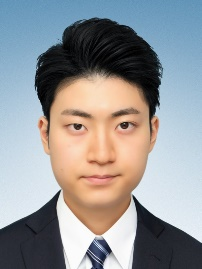
\includegraphics[width=1in,height=1.25in,clip,keepaspectratio]{自分の画像.jpg}}]{Yuminosuke Sato}
        was born on October 8, 2000,
        in Ibaraki, Japan. I completed my Bachelor's degree
        in Computer Science from the University of Aizu in
        2022 and am currently pursuing my Master's degree
        in the same field at the same university. My primary
        research focus is on the analysis and application of
        brainwave signals. In my work, I delve deeply into
        the nuances of brainwave signal interpretation and
        its potential applications. This focus has positioned
        me at the leading edge of emerging research in this
        area, leading to new discoveries and technological breakthroughs. While I
        have not yet engaged extensively in professional society activities, I am
        considering involvement in organizations such as the IEEE. My dedication
        to advancing knowledge and technology in my field showcases my potential
        as an emerging scholar, with a strong commitment to contributing to societal
        advancement through academic research.
    \end{IEEEbiography}
    \begin{IEEEbiography}
        [{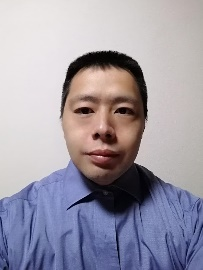
\includegraphics[width=1in,height=1.25in,clip,keepaspectratio]{矢口先生写真.jpg}}]{YUICHI YAGUCHI}
        is currently a Senior Associate Professor at the School of Computer Science and Engineering at the University of Aizu, Japan. His research interests include drone formation flight, cloud robotics, SLAM, 3-D reconstruction from aerial images, and drone automatic control. He is also a member of ISO TC20/SC16/WG4 as a Japan expert.
    \end{IEEEbiography}

    \EOD
\end{document}
